% !TEX root = ../main.tex
% Appendix D

\chapter{Testing the reduced speed of light approximation} % Main appendix title

\label{AppendixD} % For referencing this appendix elsewhere, use \ref{AppendixD}

% Variable speed of light simulations----------------------------------------------------------------------------------------
Pure--hydrodynamical simulations are very fast and due to the parallelization of the code, core collapses of several free--fall times can be finished within hours on 128 cores.
If radiative transfer is added to the simulations, the duration of runs can expand to days or months even with multiple cores.
This calls for optimization methods in the radiative transfer solver.

In the following, simulations are presented investigating methods with exactly this purpose.
They start from the same initial conditions as described by \secref{subsec:Initial_conditions}.
The RT parameters are the same for all runs, except two parameters, which are varied once at a time.
To be specific, the parameter space spanned by \code{rt\_nsubcycle} and \code{c\_frac\_speed\_factor} has been tested for the values [100, 10, 1]$\otimes$[0.1, 1.0, 10.0].

\subsubsection{Correction factor}
In the official RAMSES--RT parameters, the reduced speed of light approximation is set from start and not changed during the simulation.
An as of yet unofficial RAMSES--RT routine involving the parameter \code{c\_frac\_speed\_factor} implements another approach.
With it, the initial fraction of the reduced speed of light (here representatively called \code{new\_rt\_c}) and the actual speed of light is constraint by the global maximal gas velocity, the sound speed and the maximal optical depth in the simulation box.
\begin{equation*}
  \code{new\_rt\_c = c\_frac\_speed\_factor * max(u\_gas\_abs, c\_sound) * max(tau, 1.)}
\end{equation*}
The maximal optical depth \code{tau} and fluid velocity \code{u\_gas\_abs} are evaluated within every MPI--domain and their global maxima are subsequently determined with an \code{MPI\_ALLREDUCE} call.
Thus, whenever a new and higher optical depth or flow velocity occurs in the simulation, the reduced speed of light is updated.

\subsubsection{RT subcycling}
The subcycling of the radiative transfer routine with \code{rt\_nsubcycle} provides a faster solution for very stiff source terms in the thermochemistry steps.
If the optical depth in a simulation is extremely high, the source terms become very stiff and the subcycling the routine might never converge to a solution.
By introducing a limiting step number \code{rt\_nsubcycle} the subcycling is stopped by avoiding further unnecessary steps at an almost converged solution.

Further details on the exact values of the parameters of the simulation runs can be found in the overview in Appendix~\ref{sec:Overview} in Table \ref{tab:var_rt}.
Upon evaluation of the runs' durations, the variable RSLA was regarded unecessary and abandoned afterwards.

\subsubsection{Effects of the parameters}
\figref{fig:var_rt_profile} shows the resulting density and temperature profiles of such a run, with parameters \code{rt\_nsubcycle=1} and \code{c\_frac\_speed\_factor=10.}
There still is a remainder of the singular isothermal sphere profile recognizable, but with some outliers due to secondary sinks on a stable orbit around the center, amassing gas around them.
Near the center, there is also a drop in density, which can be explained by the fast accretion of the central sink, creating a vacuum.
The density of the sinks themselves is not accounted for in these profiles.
The influence of infrared radiation is also clearly visible.
Within an effective radius of around 1000 AU the accretion luminosity of the sink heats up the gas around it and rises the temperature floor of the ISM of 10 Kelvin to roughly 30 to 40 Kelvin.
\\[6pt]
%
While the profiles show thermodynamical properties along the radius of the disk averaged over $2\pi$ radians, it is also interesting to directly compare these properties.
Phase space diagrams have exactly this purpose.
\figref{fig:var_rt_larson_rhoT} shows such a phase space diagram of the same simulation as before (\code{nsub1c10}).
The results are what was expected, similar to \citet{Commercon_collapse} or \citet{Larson_paper}.
At low densities, most of the mass seems to quite efficiently cool down to the floor level of around 10 K.
After the first Larson core formed, the collapse progresses quasi--adiabatically.
At higher densities, the optical depth rises and with it the temperature.

The same and similar plots for the runs in Table \ref{tab:var_rt} with other values for the parameters are found in the Appendix \ref{AppendixD}.

A curious case can be found in runs with lower values of \code{c\_frac\_speed\_factor}.
Here, the lower densities can also be heated up to the same level as gas in the optically thick regime.
A possible explanation for this could be the accretion of sink particles.
Due to the sink's accretion, low--density regions develop around the sink, and its luminosity combined with the low reduced speed of light causes these regions to heat up.

\begin{figure*}[!htb]
 \centering
 %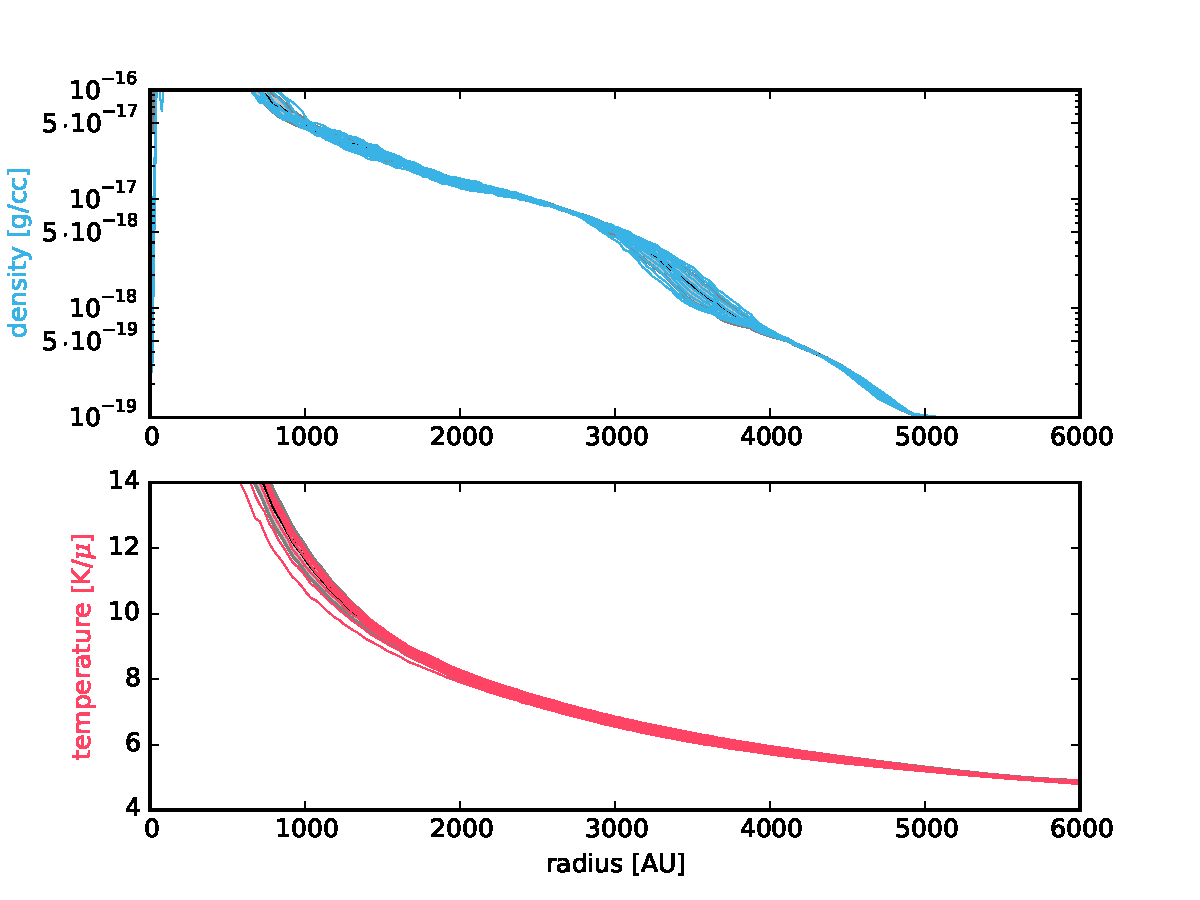
\includegraphics[width=0.99\textwidth]{Figures/var_rt_profiles/timeave_n100c01_6000AU}
 %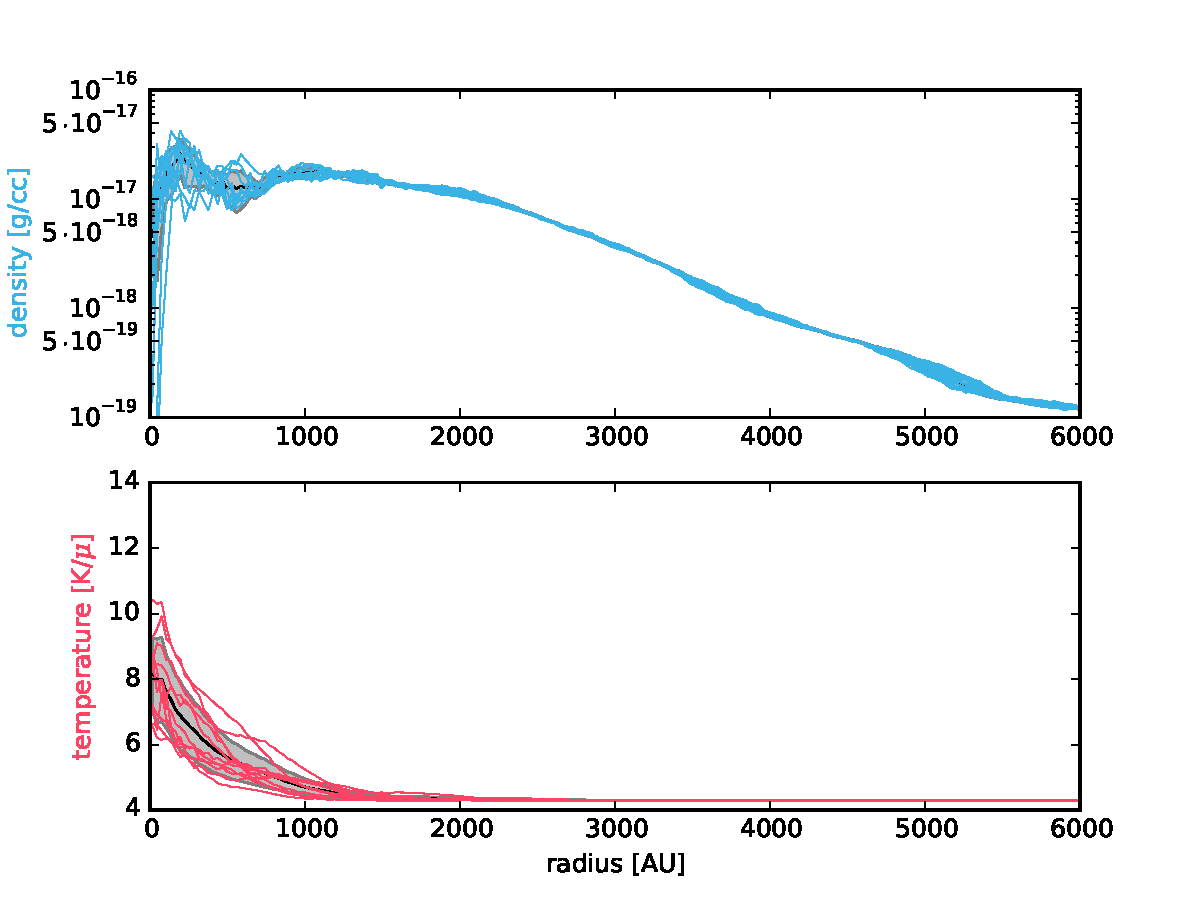
\includegraphics[width=0.99\textwidth]{Figures/var_rt_profiles/timeave_n100c1_6000AU}
 %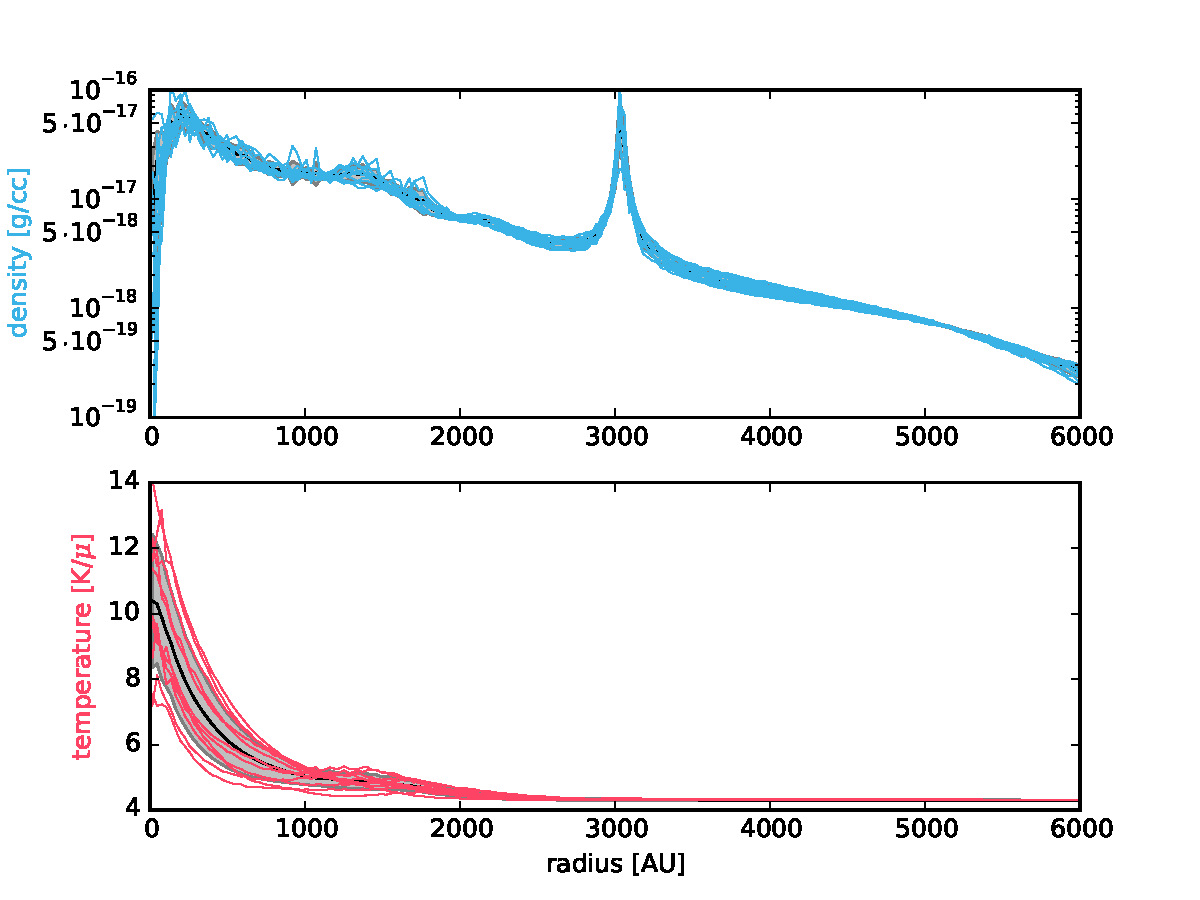
\includegraphics[width=0.99\textwidth]{Figures/var_rt_profiles/timeave_n100c10_6000AU}
 %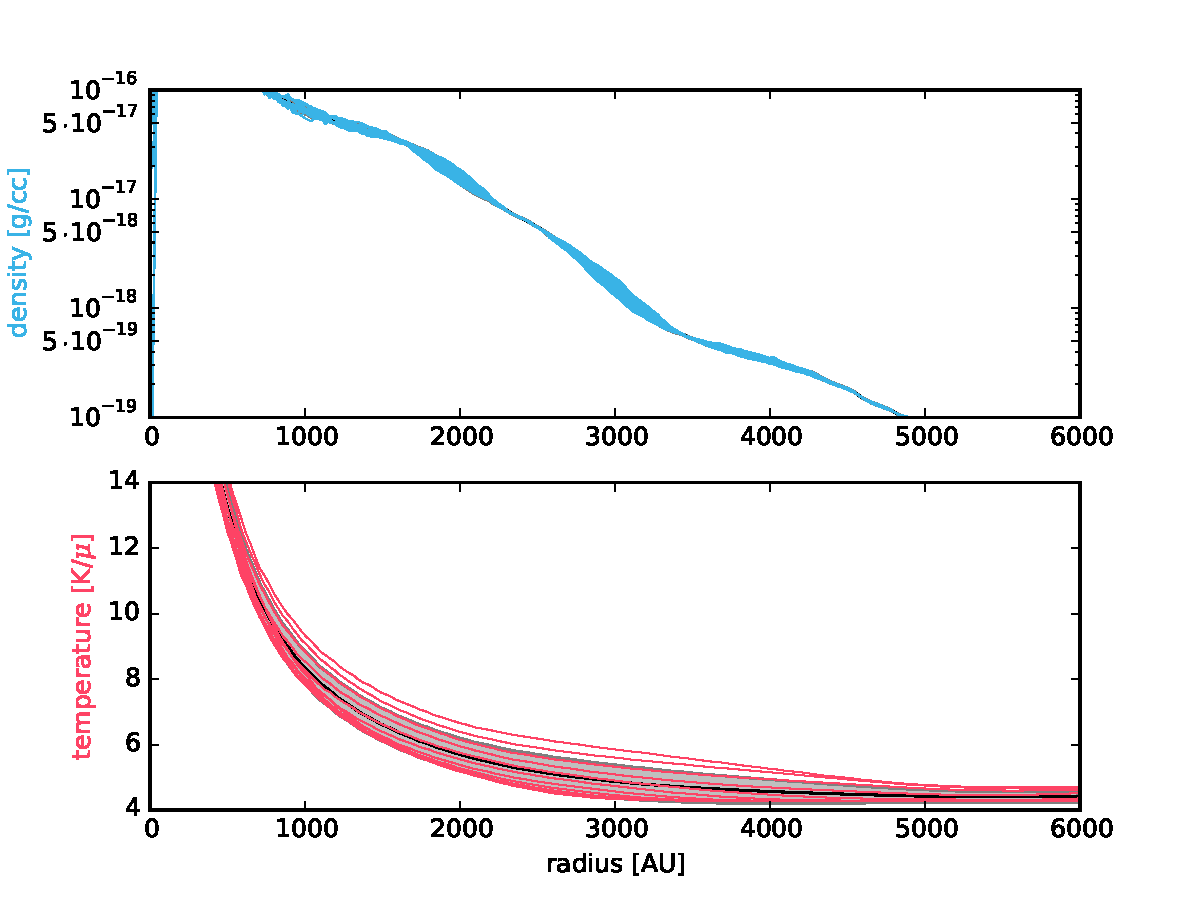
\includegraphics[width=0.99\textwidth]{Figures/var_rt_profiles/timeave_n10c01_6000AU}
 %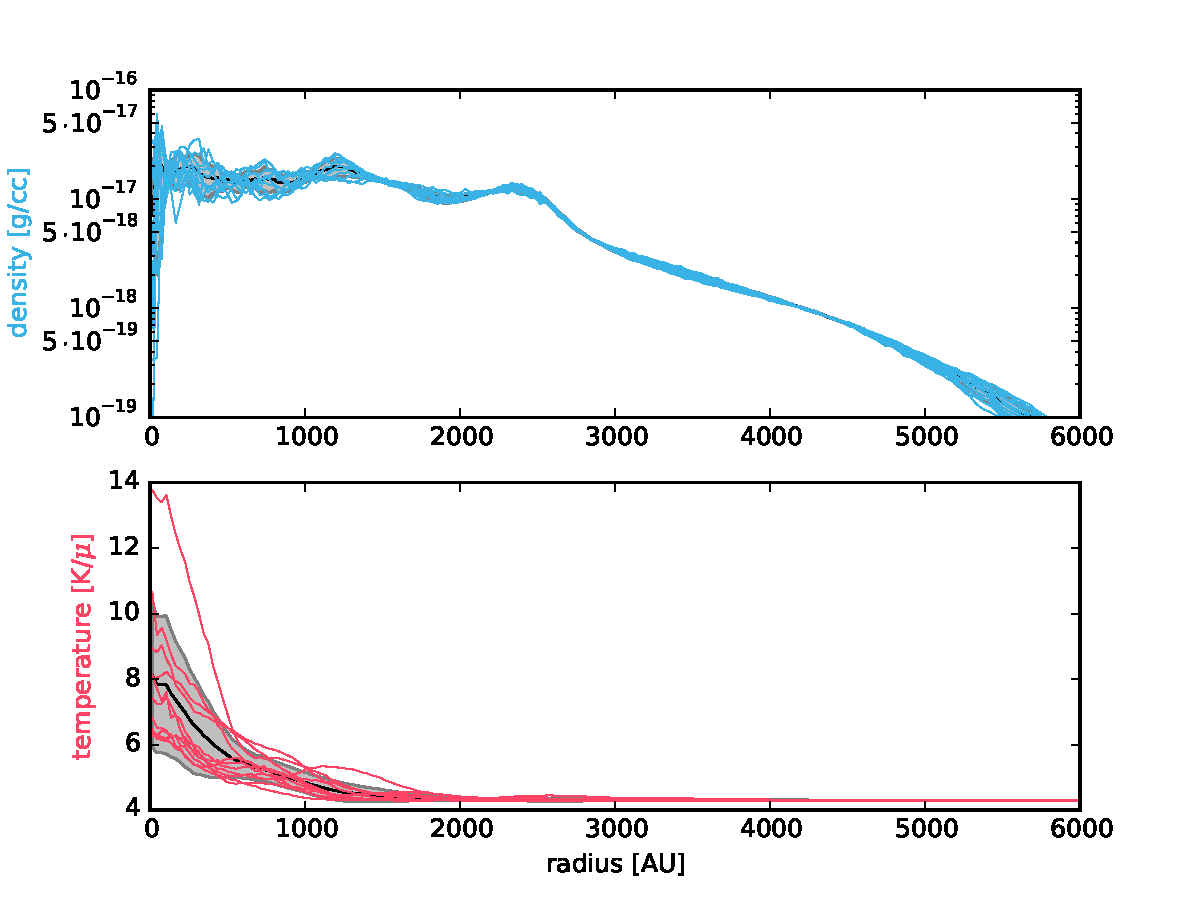
\includegraphics[width=0.99\textwidth]{Figures/var_rt_profiles/timeave_n10c1_6000AU}
 %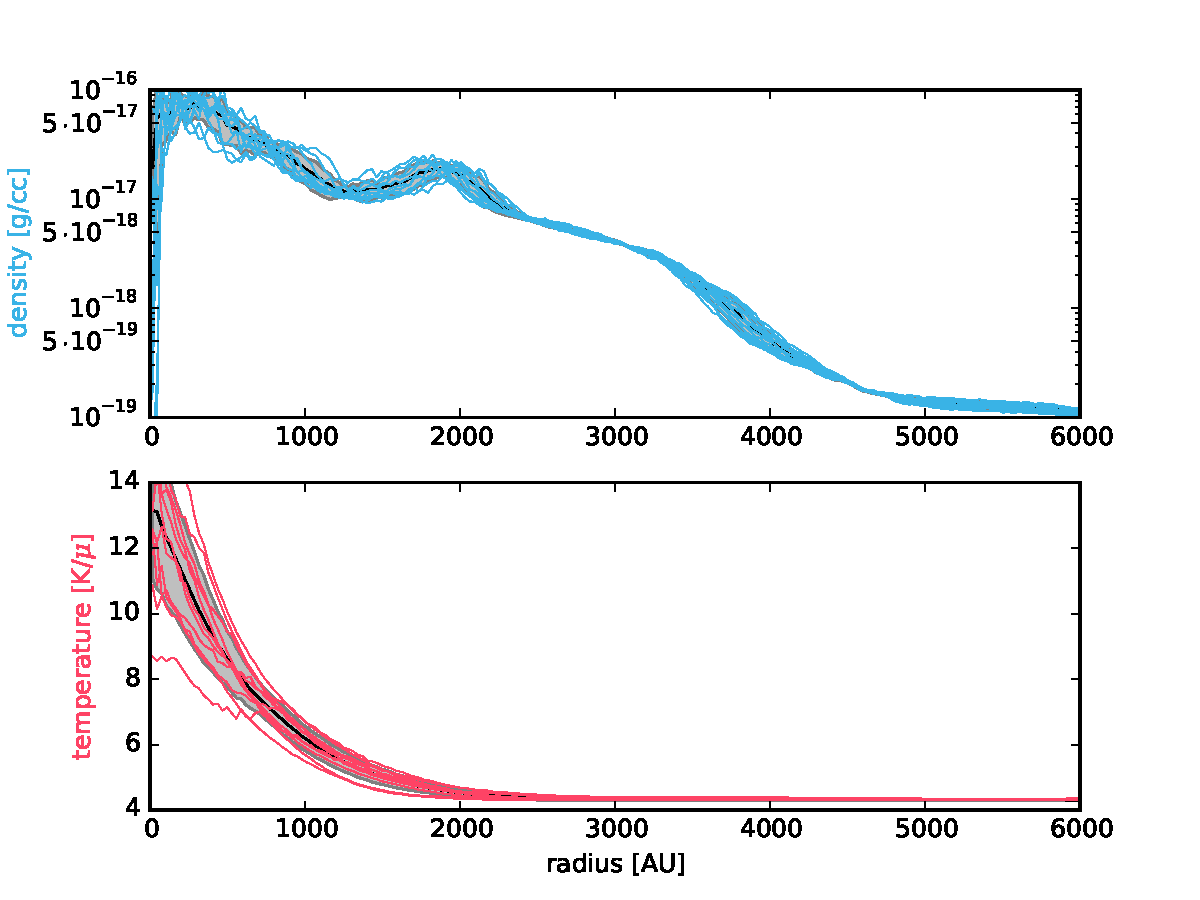
\includegraphics[width=0.99\textwidth]{Figures/var_rt_profiles/timeave_n10c10_6000AU}
 %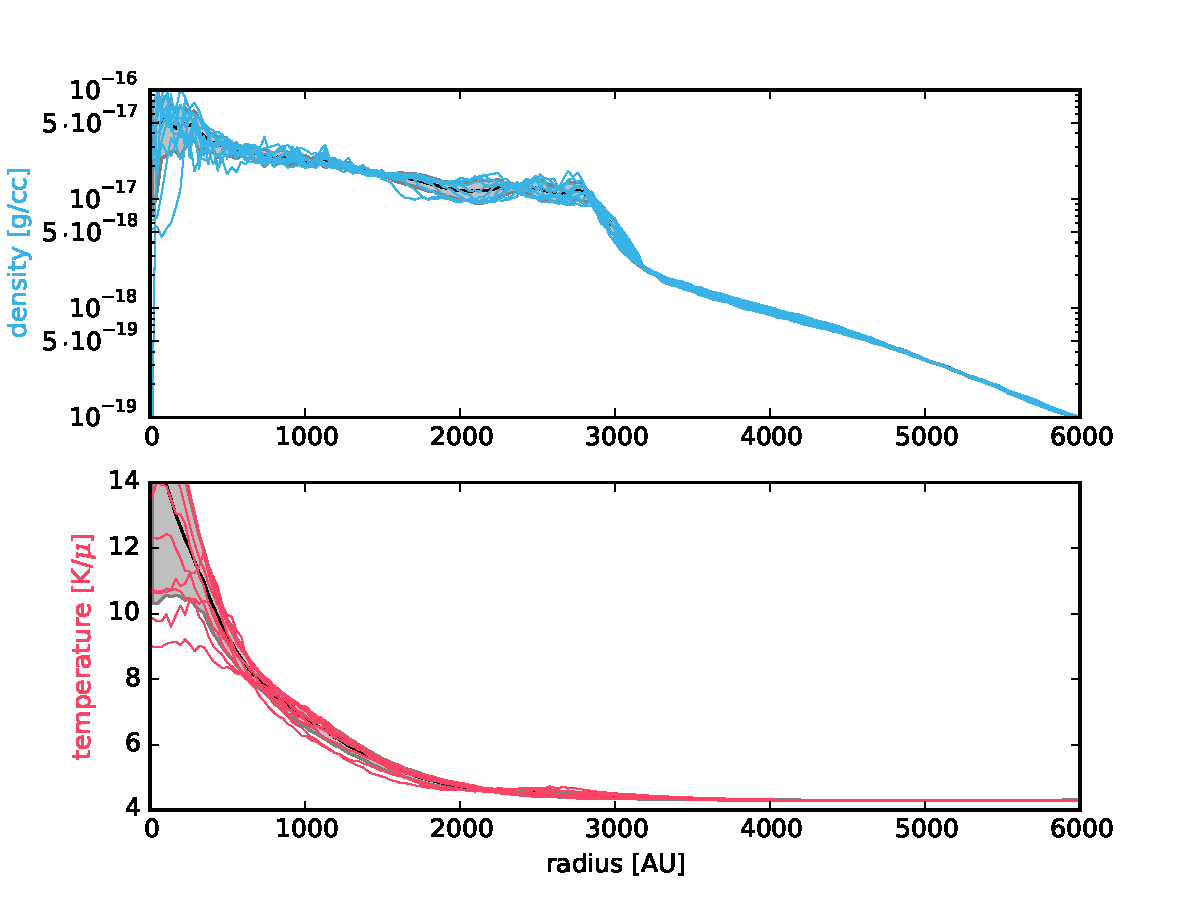
\includegraphics[width=0.99\textwidth]{Figures/var_rt_profiles/timeave_n1c01_6000AU}
 %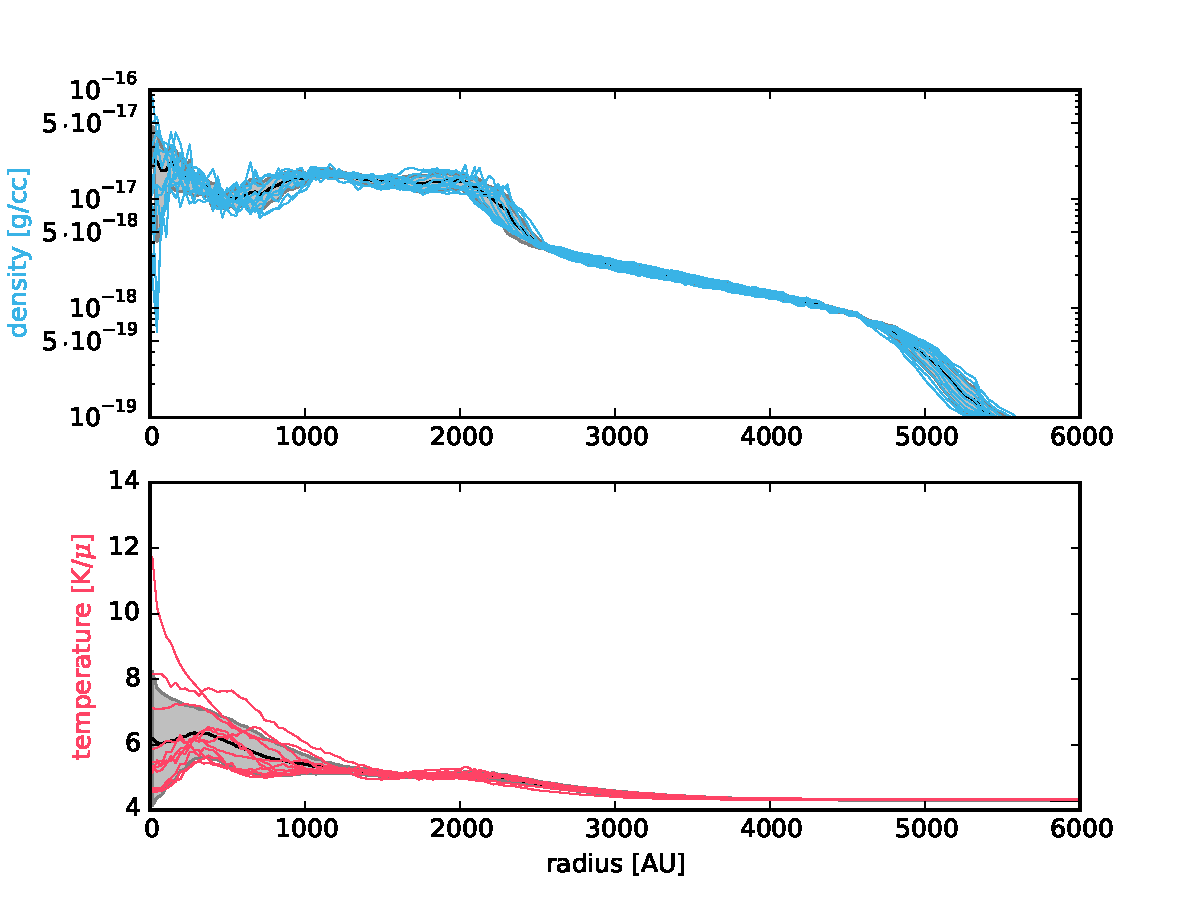
\includegraphics[width=0.99\textwidth]{Figures/var_rt_profiles/timeave_n1c1_6000AU}
 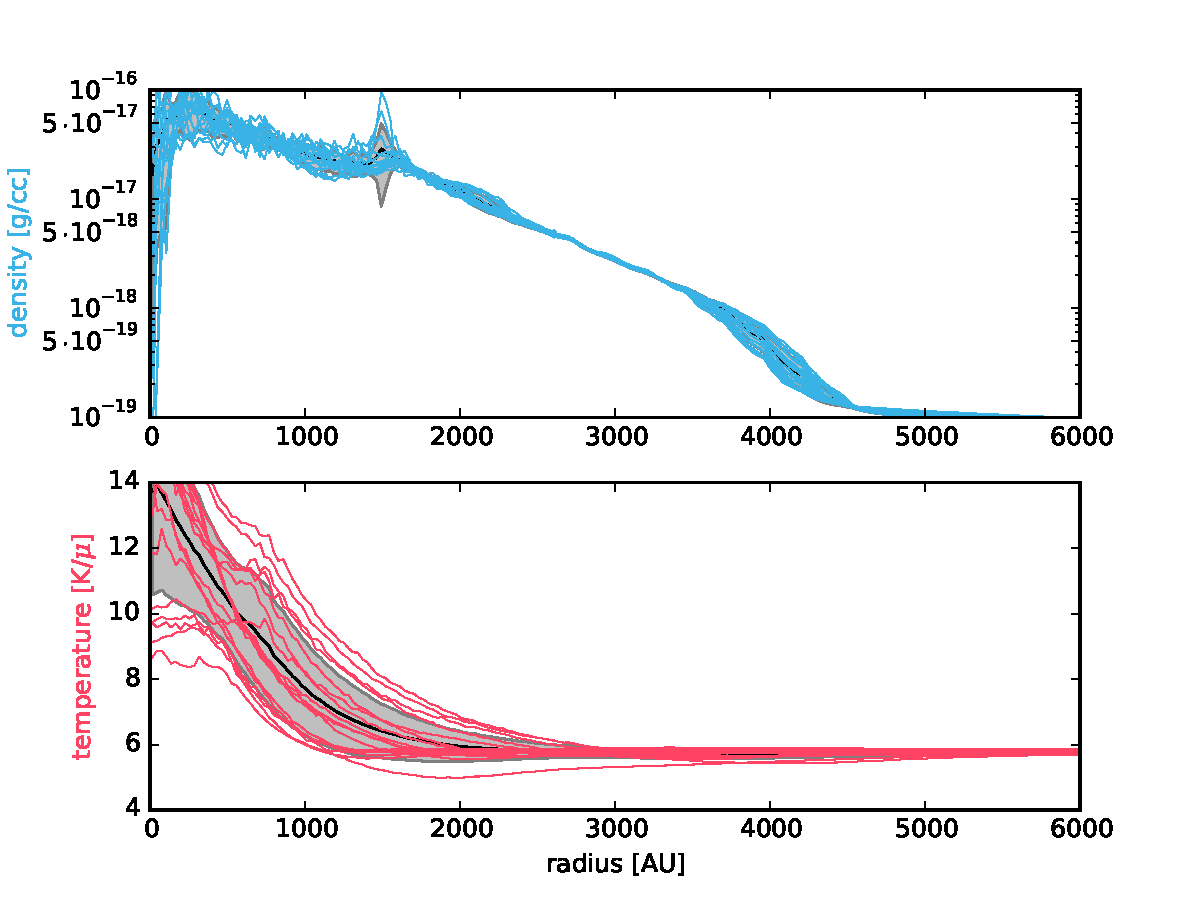
\includegraphics[width=1.0\textwidth]{Figures/var_rt_profiles/timeave_n1c10_6000AU_80_85kyrs}
 \captionsetup{justification=justified,singlelinecheck=false,width=\linewidth}
 \decoRule
 \caption[Density and temperature profiles]{Density and temperature profiles of \code{nsub1c10} run.
                                            The blue/red lines show the density/temperature profiles calculated at the last ten snapshots of the simulation at 80.49 to 85.50 kyrs.
                                            A grey--shaded area denotes the variance around the time--averaged value drawn as a black line.
                                            $\mu$ (with a value of around 2.3) denotes the molecular weight of the gas admixture of H, HII, H$_{2}$, and He.
                                            Centered around the most massive sink, a million points were randomly sampled within a radius of 6000 AU and a disk height of a few AU.
                                            These points were then histogrammed within concentrical shells.}
\label{fig:var_rt_profile}
\end{figure*}
\FloatBarrier

\begin{figure*}[!htb]
 \centering
 %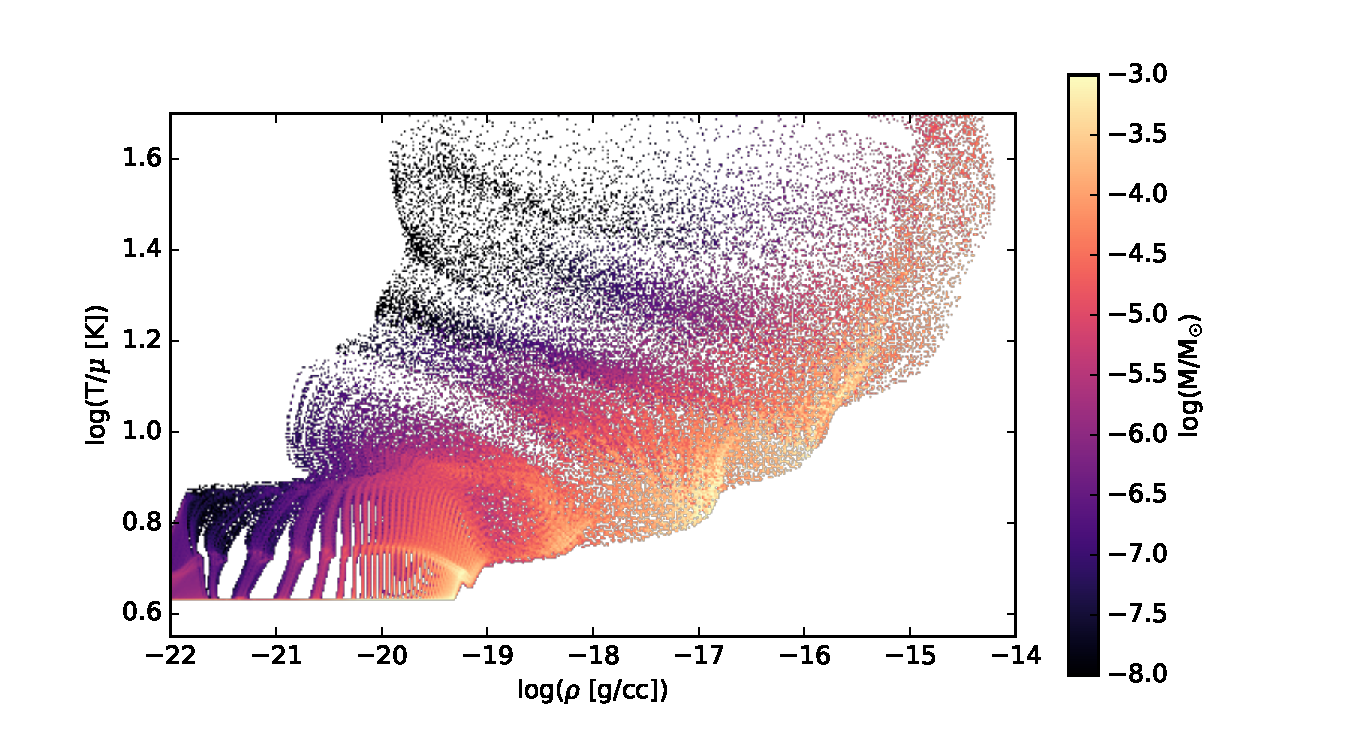
\includegraphics[width=0.99\textwidth]{Figures/var_rt_larson_plots/rho_temp_hist_n100c01}
 %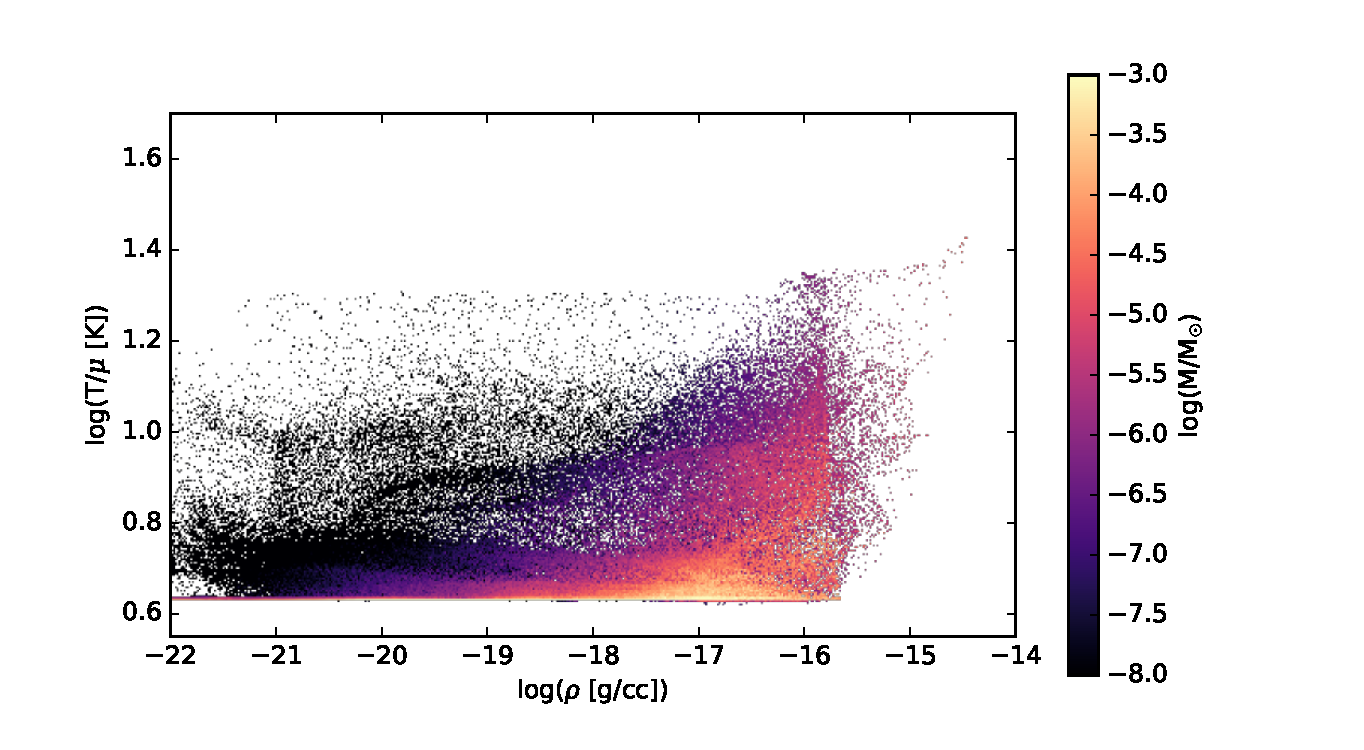
\includegraphics[width=0.99\textwidth]{Figures/var_rt_larson_plots/rho_temp_hist_n100c1}
 %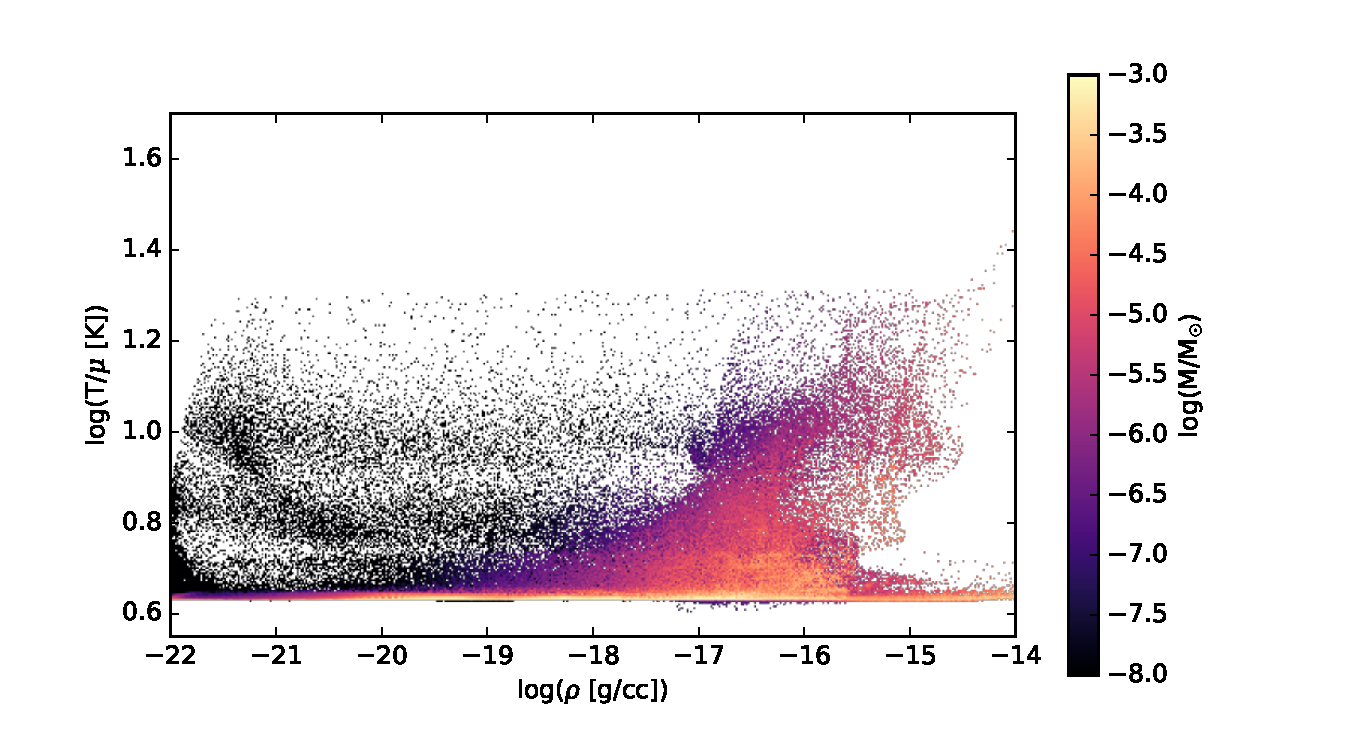
\includegraphics[width=0.99\textwidth]{Figures/var_rt_larson_plots/rho_temp_hist_n100c10}
 %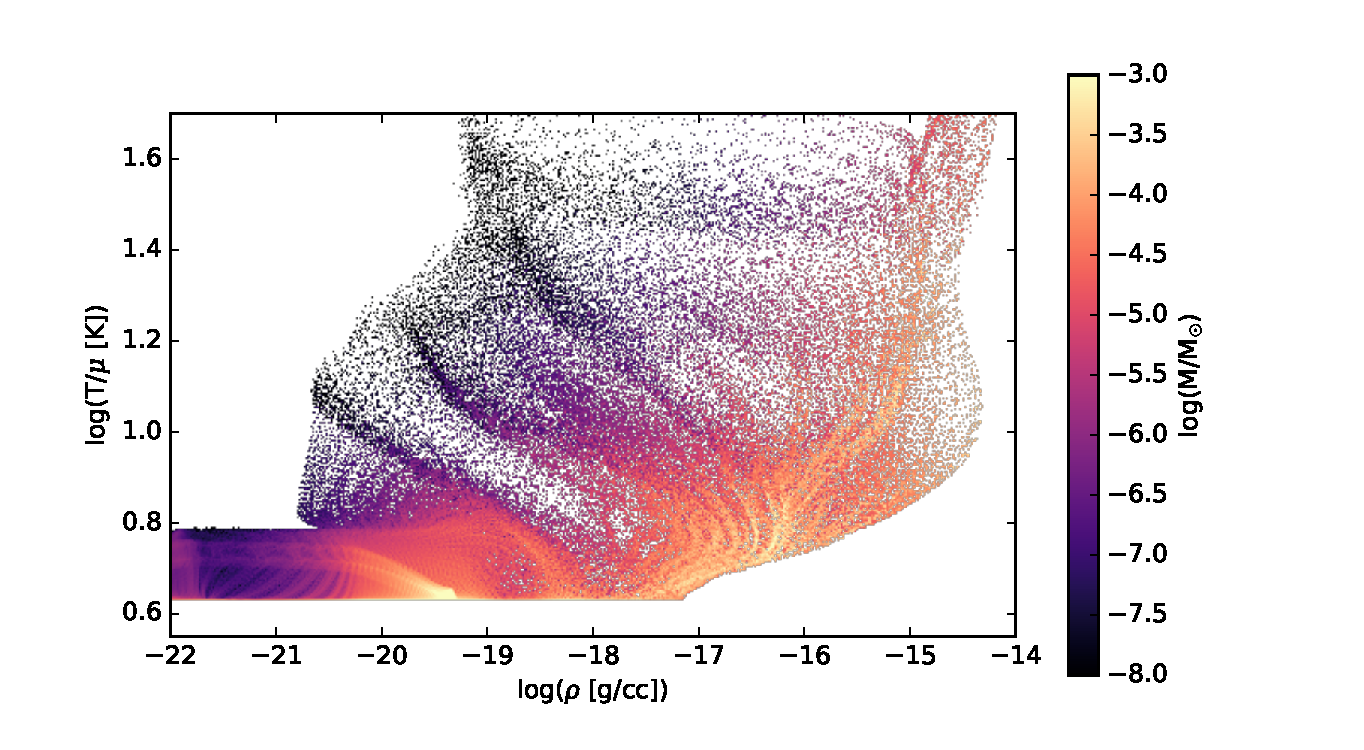
\includegraphics[width=0.99\textwidth]{Figures/var_rt_larson_plots/rho_temp_hist_n10c01}
 %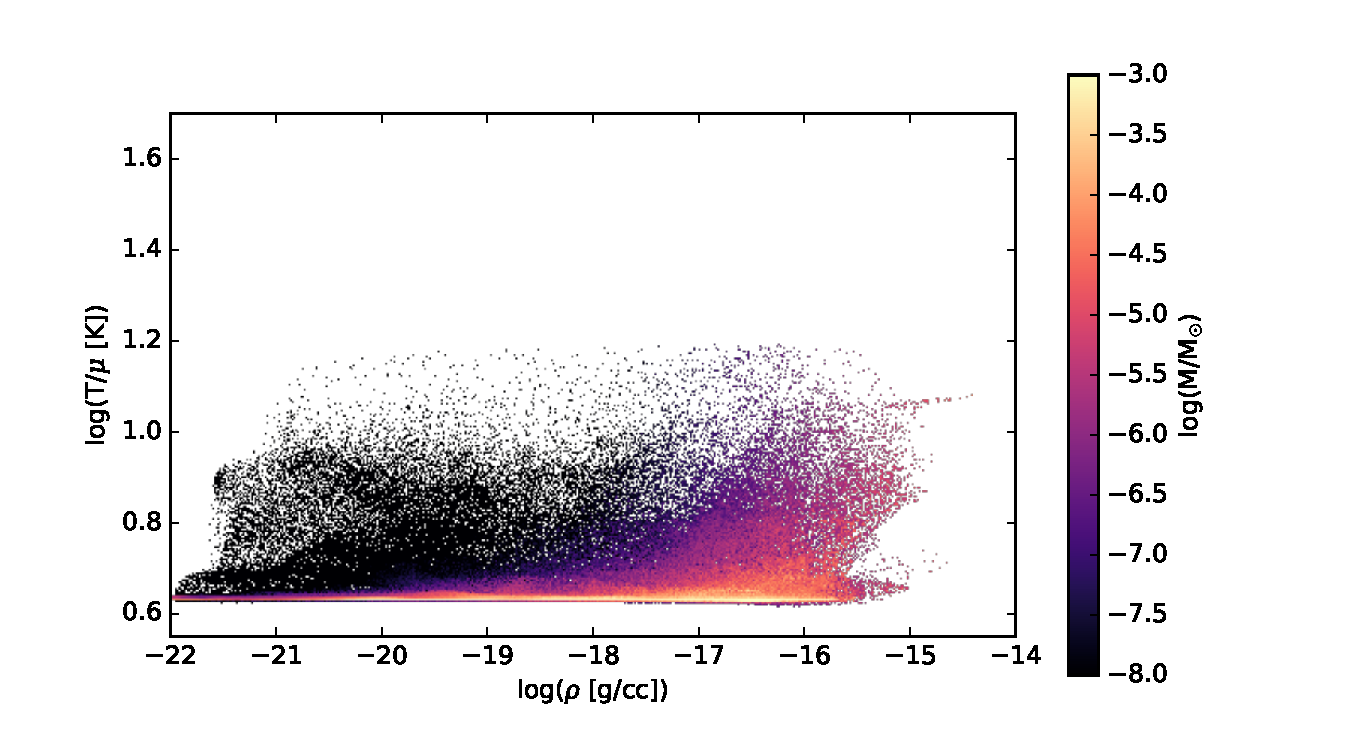
\includegraphics[width=0.99\textwidth]{Figures/var_rt_larson_plots/rho_temp_hist_n10c1}
 %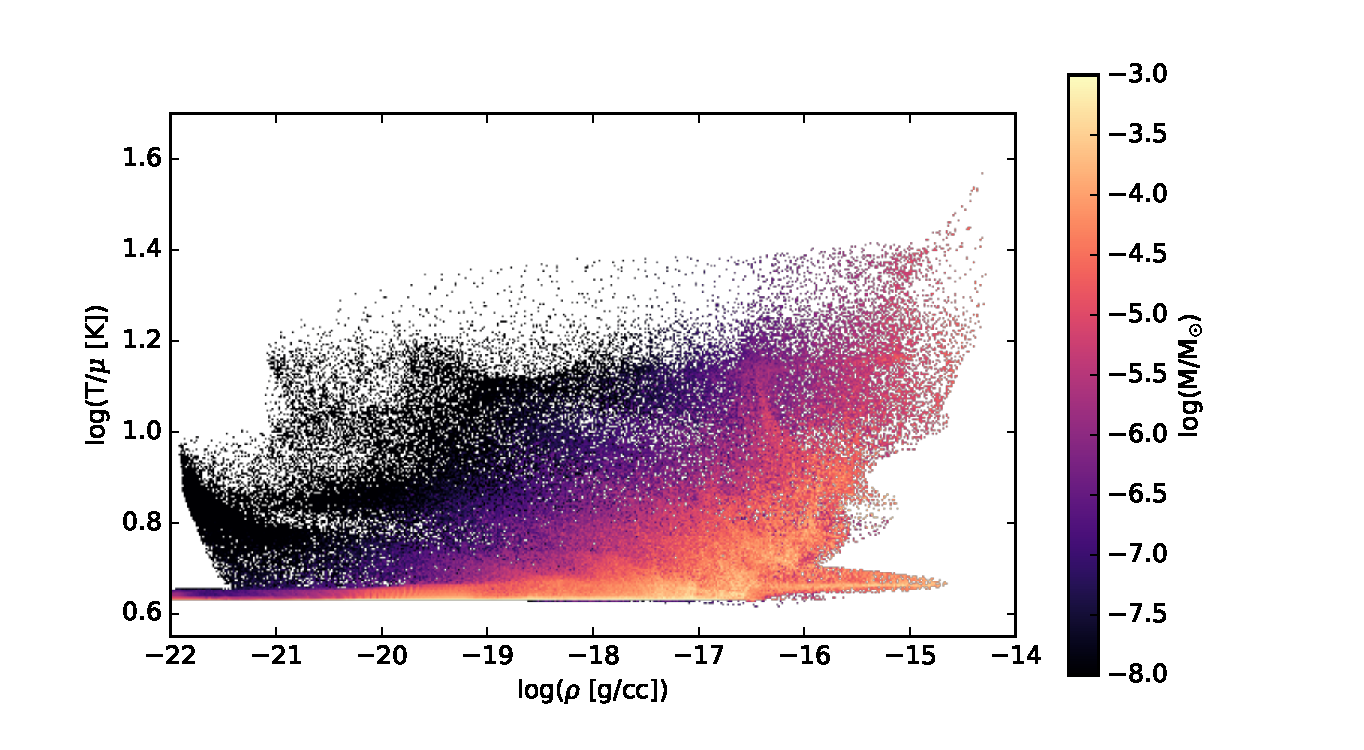
\includegraphics[width=0.99\textwidth]{Figures/var_rt_larson_plots/rho_temp_hist_n10c10}
 %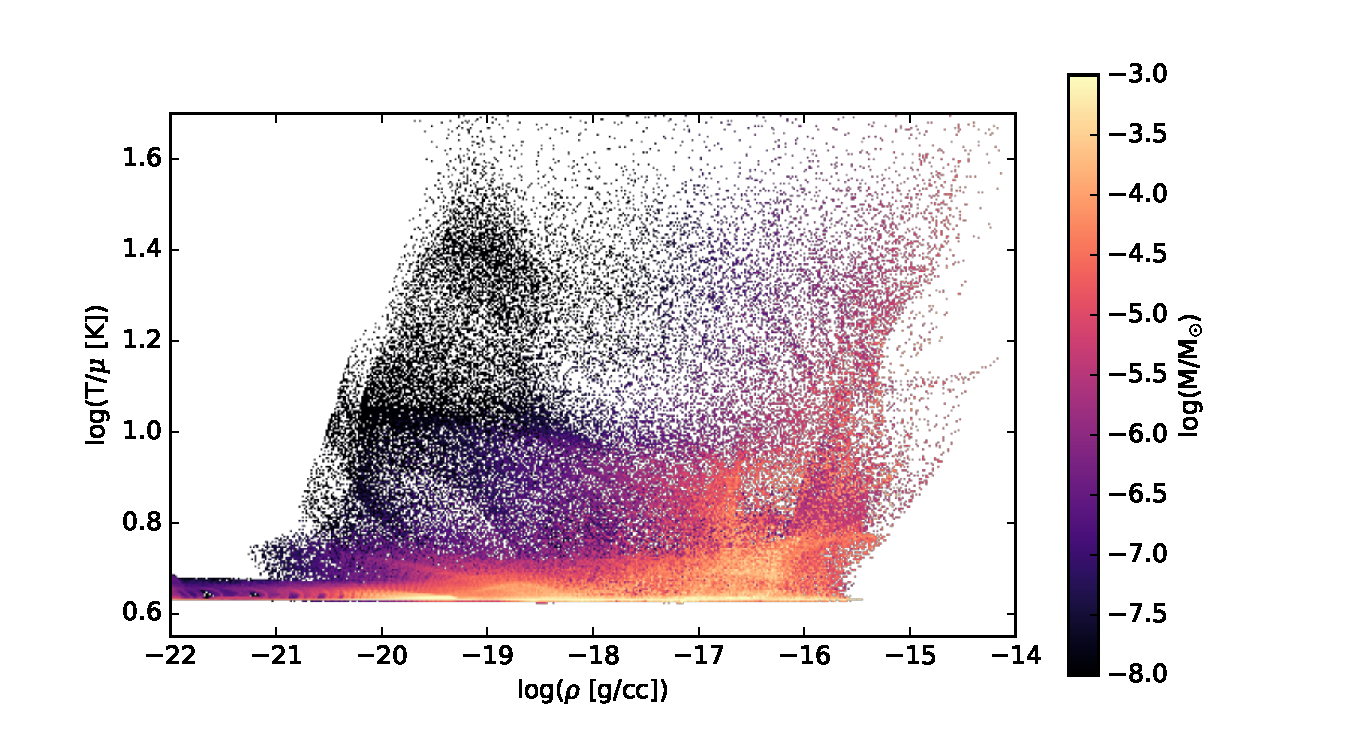
\includegraphics[width=0.99\textwidth]{Figures/var_rt_larson_plots/rho_temp_hist_n1c01}
 %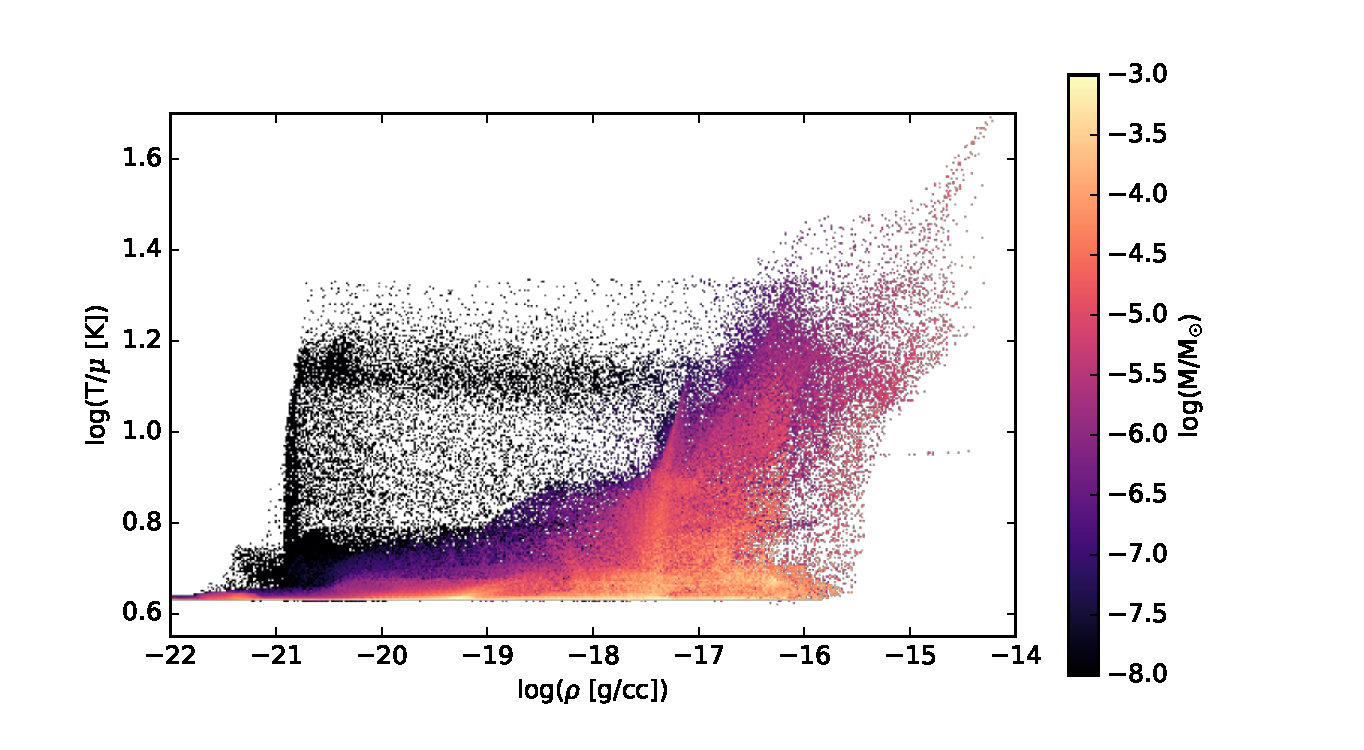
\includegraphics[width=0.99\textwidth]{Figures/var_rt_larson_plots/rho_temp_hist_n1c1}
 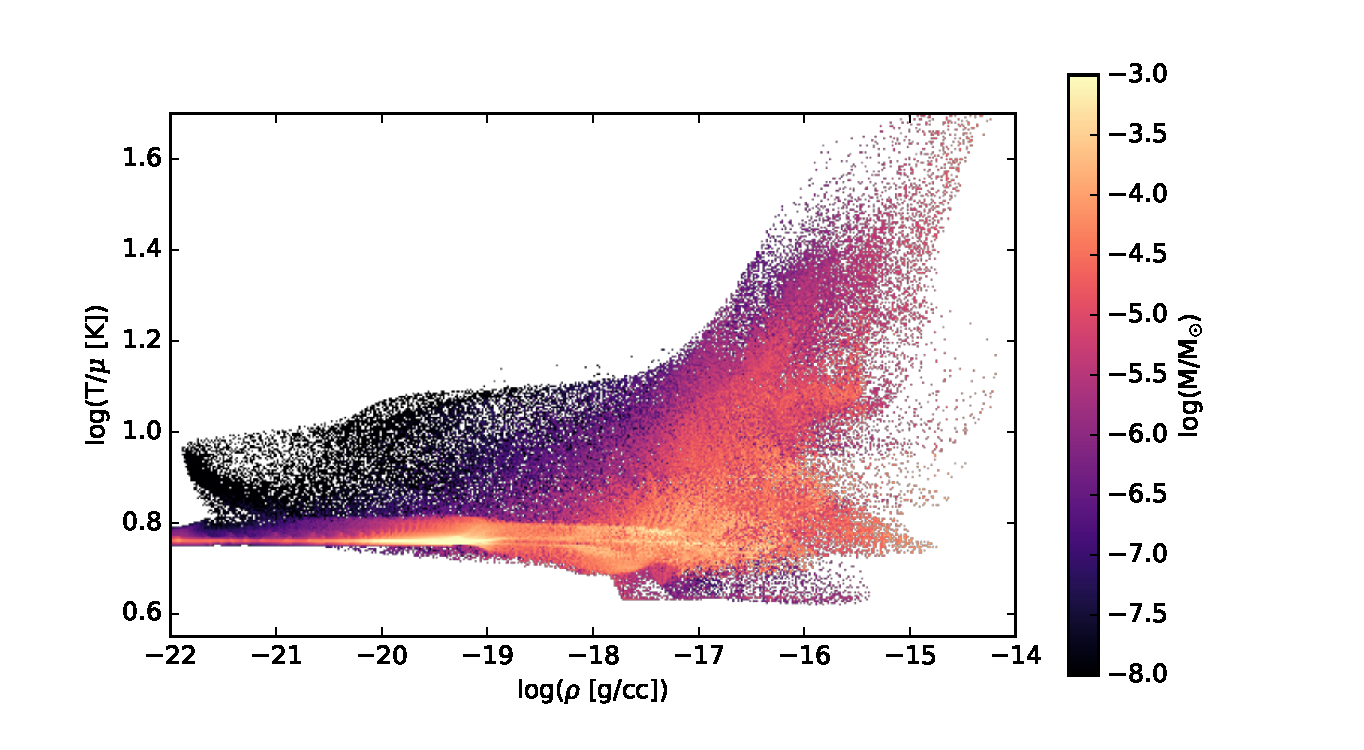
\includegraphics[width=1.0\textwidth]{Figures/var_rt_larson_plots/rho_temp_hist_n1c10}
 \captionsetup{justification=justified,singlelinecheck=false,width=\linewidth}
 \decoRule
 \caption[$\rho$--T phase diagram]{Density--temperature phase space diagram of \code{nsub1c10} run at 85.50 kyrs.
 %TODO
                                   Most of the mass follows on average the profile described by a polytropic EOS; see \secref{sec:Reference_runs}.
                                   At a knee density determined by the point where the optical depth crosses the opacity limit $\tau \simeq 1$, the radiation starts to become trapped and heats up the gas.
                                   At this point the first Larson core has formed; see \secref{subsec:Larson_cores}.}
\label{fig:var_rt_larson_rhoT}
\end{figure*}
\FloatBarrier


% other profiles ----------------------------------------------------------------------------------------
\subsubsection{Compilation of further profiles}
Here, all density and temperature profiles from the runs with variable reduced speed of light are shown.
The profiles are calculated within a disk radius of 6000 AU centered around the most massive sink in each simulation.
Within a relatively low disk height, a million sampling points are randomly selected and histogrammed in concentric shells.

This is done for the last ten snapshots of the simulation, which corresponds to a simulated time of 94.55 to 99.56 kyrs for all simulations, but one.
Run \code{nsub001c10} was unfortunately unable to reach the same time, since the time steps within the simulation became so small that the simulation virtually came to a halt.
Therefore the profiles for \code{nsub001c10} were calculated from a simulated time of 80.49 to 85.50 kyrs.

The blue curves show the density profiles for different snapshots, whereas the red curves show the temperature profiles for the same times.
The grey--shaded area shows the variance of the snapshots centered around the time average in black.

Another interesting analytical tool are phase space diagrams.
Phase space diagrams can show how thermodynamical properties of the simulation are related to each other.
Following the profiles, the mass--weighted phase space diagrams between density, temperature, and radius of the same runs are presented, again centered around the most massive sink.
They are calculated for every cell in a snapshot at a simulation time of 99.56 kyrs, except for the one of run \code{nsub001c10}, which was taken at 85.5 kyrs.
The radial phase space diagrams show peaks at certain radii representing sinks which accrete mass and heat up their surroundings.


% Profiles ----------------------------------------------------------------------------------------
% 0.1 c_frac_speed_factor

\begin{figure*}[!htb]
 \centering
 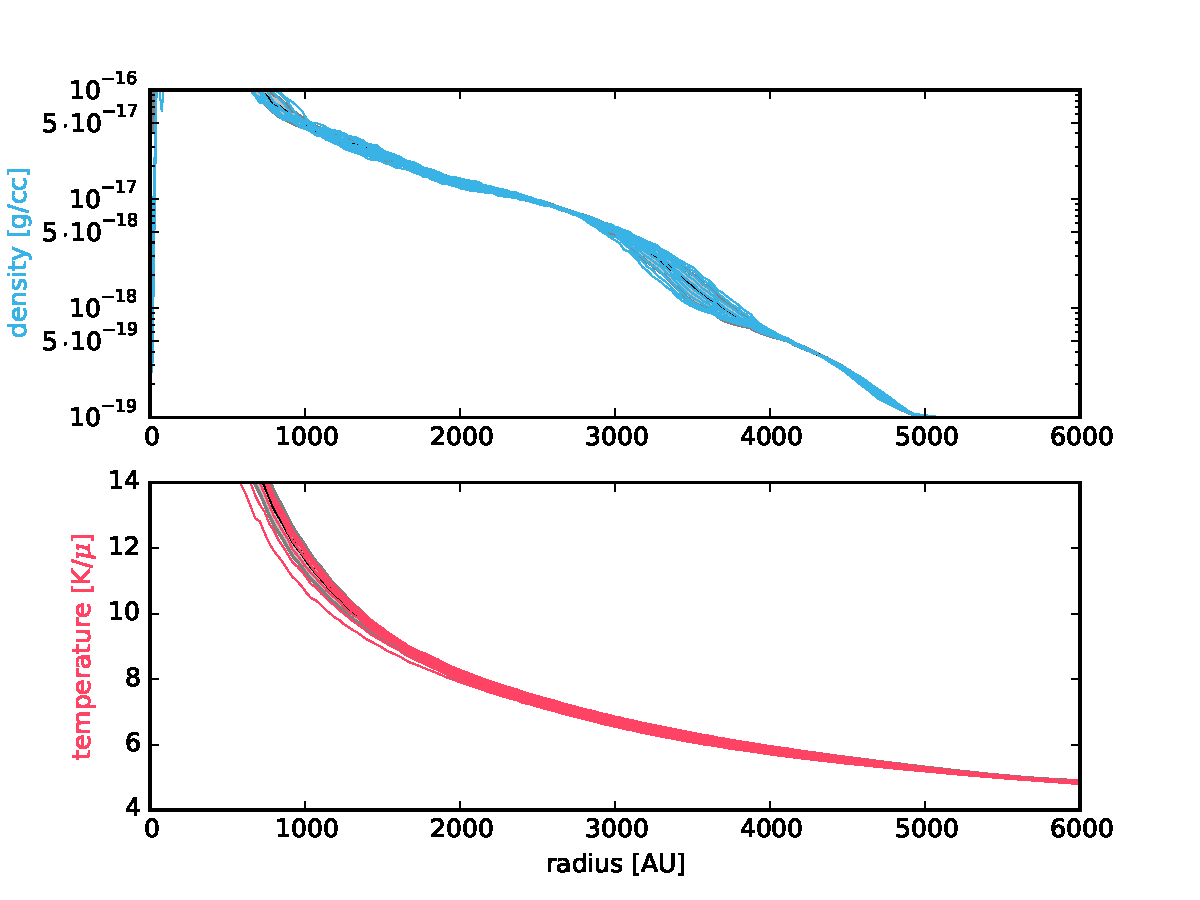
\includegraphics[width=0.95\textwidth]{Figures/var_rt_profiles/timeave_n100c01_6000AU}
 %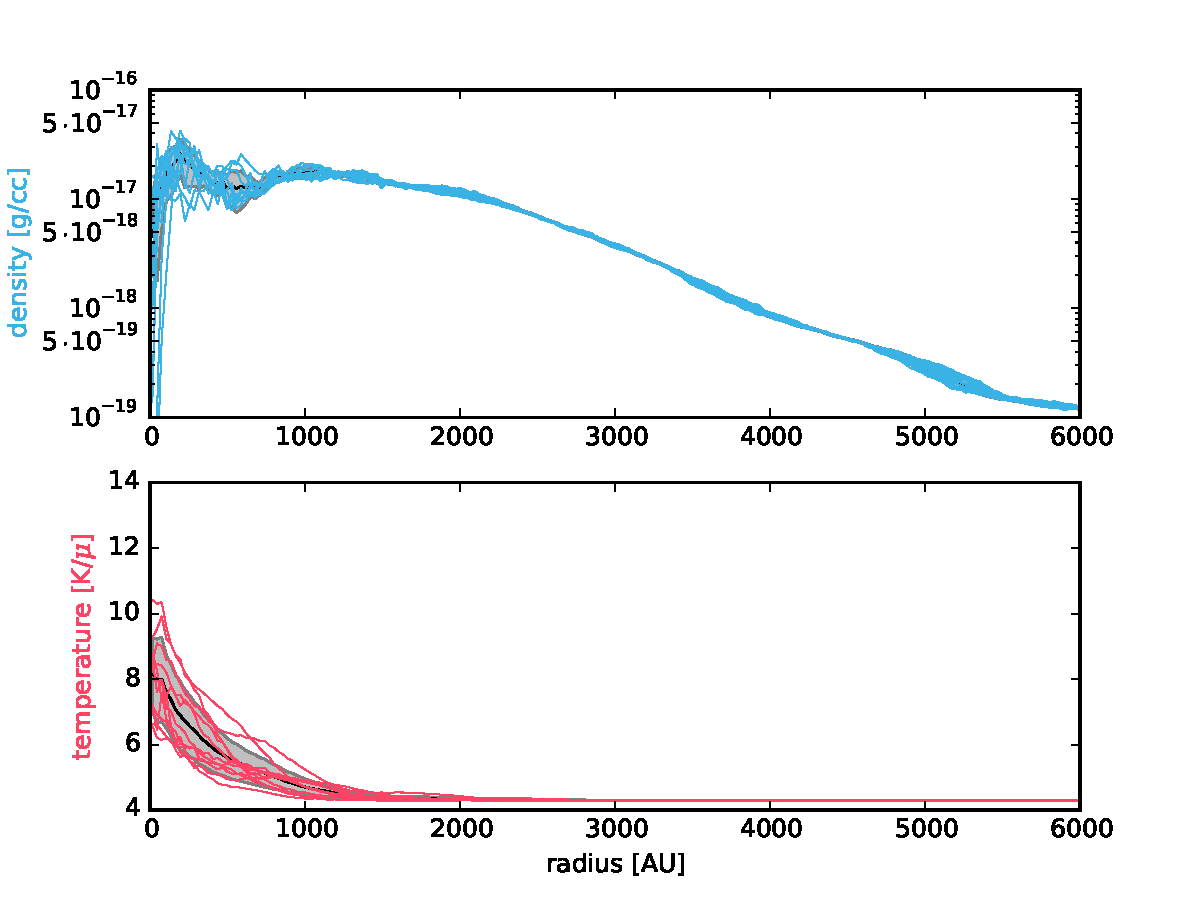
\includegraphics[width=0.99\textwidth]{Figures/var_rt_profiles/timeave_n100c1_6000AU}
 %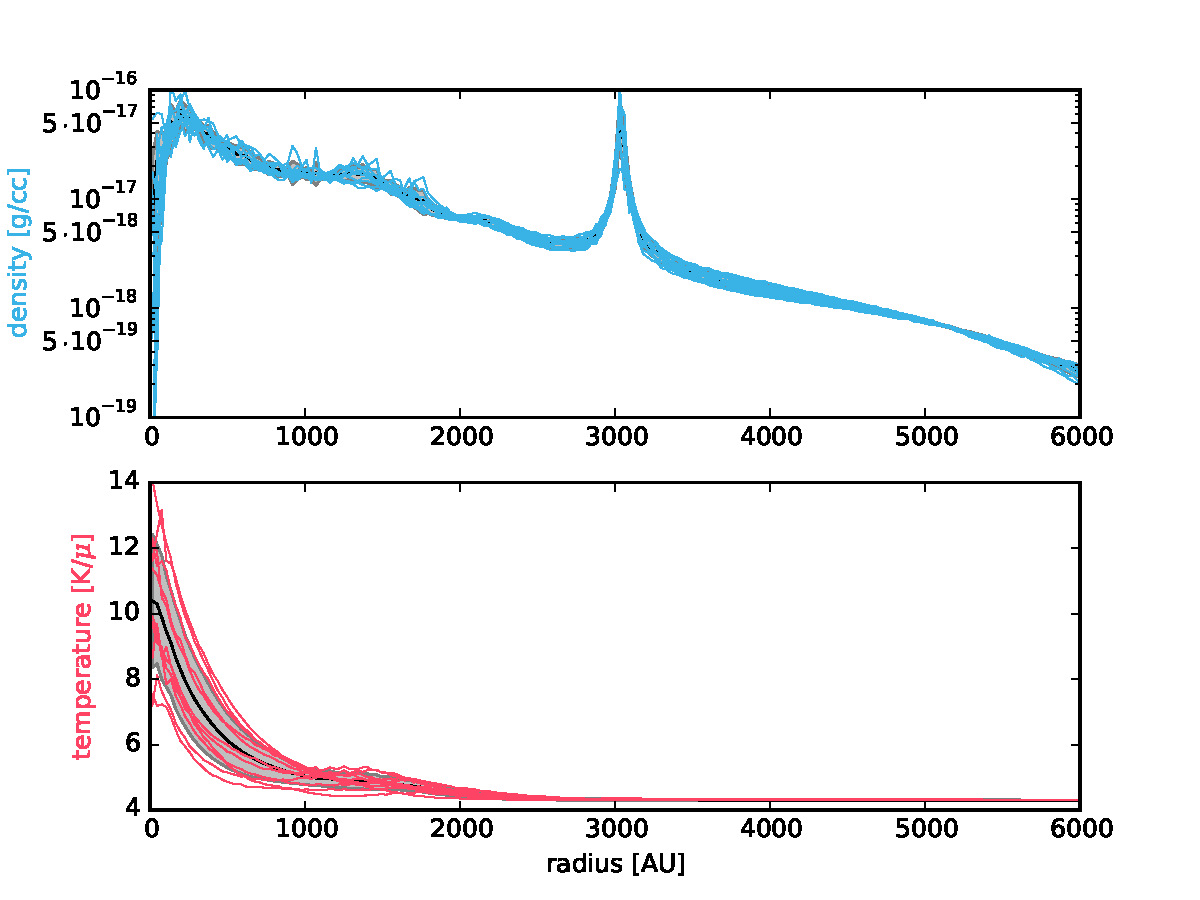
\includegraphics[width=0.99\textwidth]{Figures/var_rt_profiles/timeave_n100c10_6000AU}
 %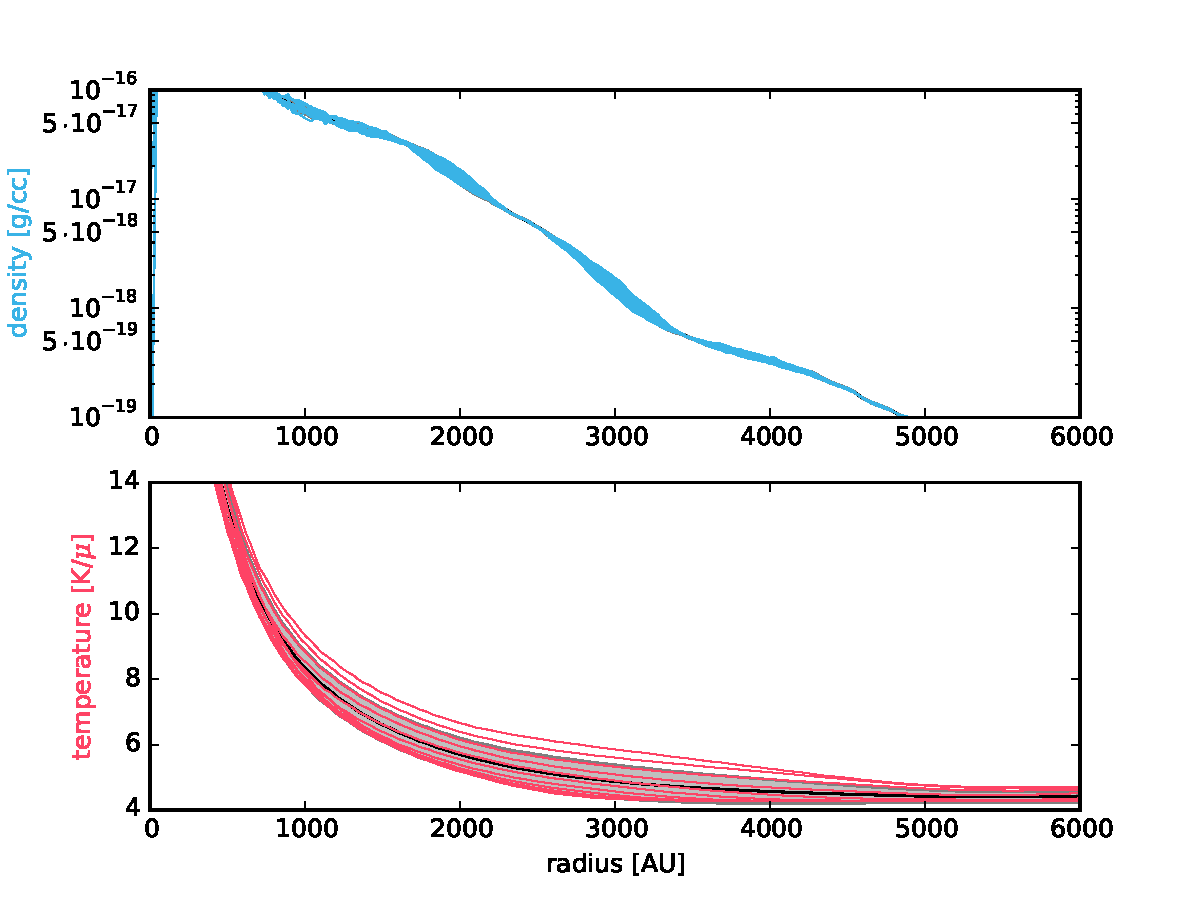
\includegraphics[width=0.99\textwidth]{Figures/var_rt_profiles/timeave_n10c01_6000AU}
 %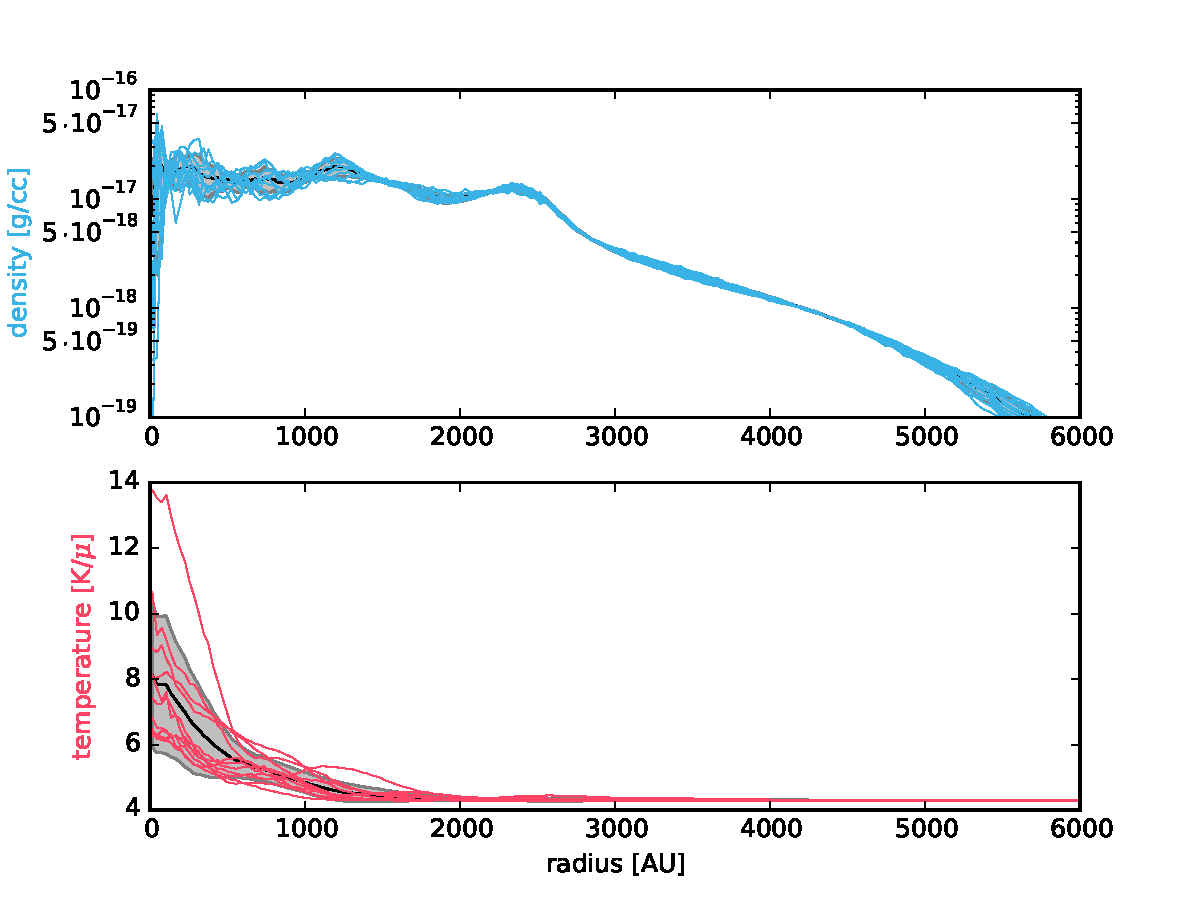
\includegraphics[width=0.99\textwidth]{Figures/var_rt_profiles/timeave_n10c1_6000AU}
 %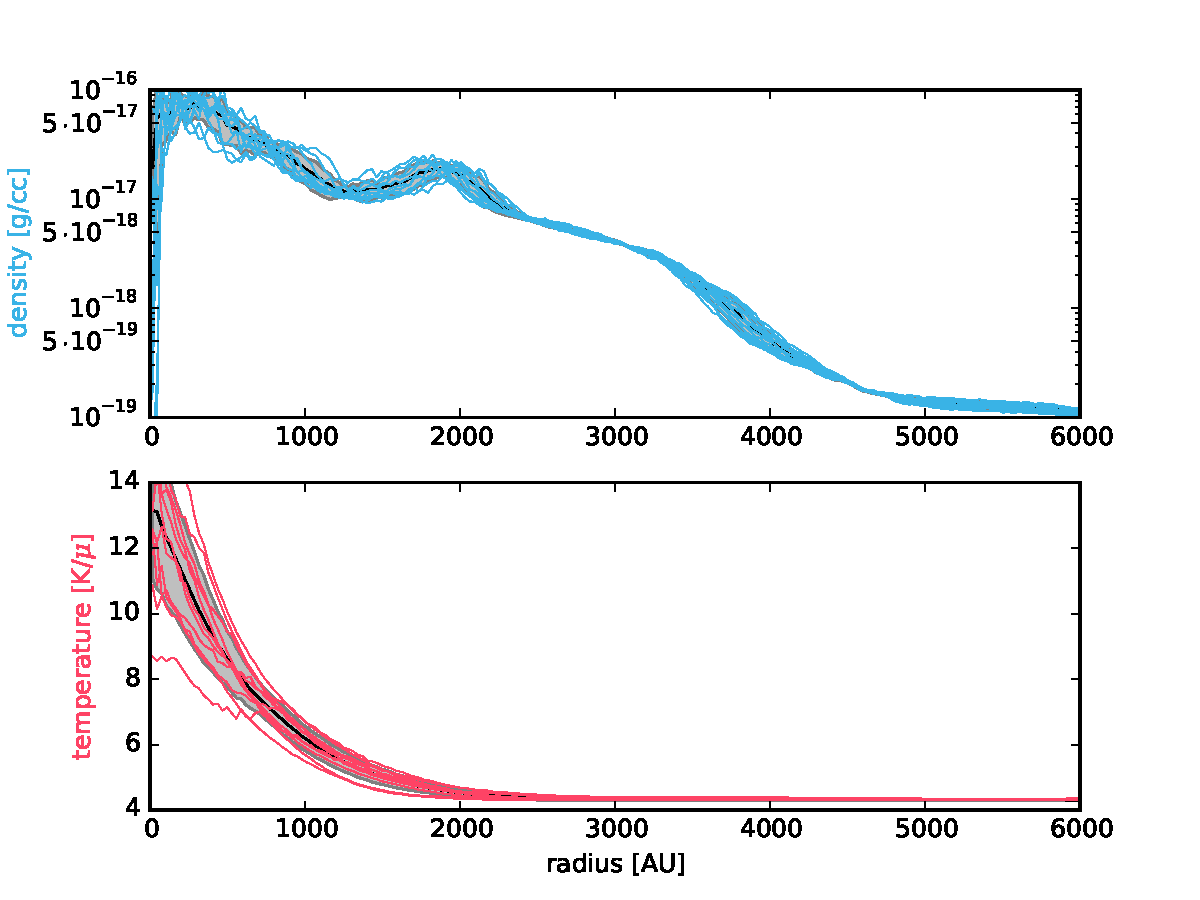
\includegraphics[width=0.99\textwidth]{Figures/var_rt_profiles/timeave_n10c10_6000AU}
 %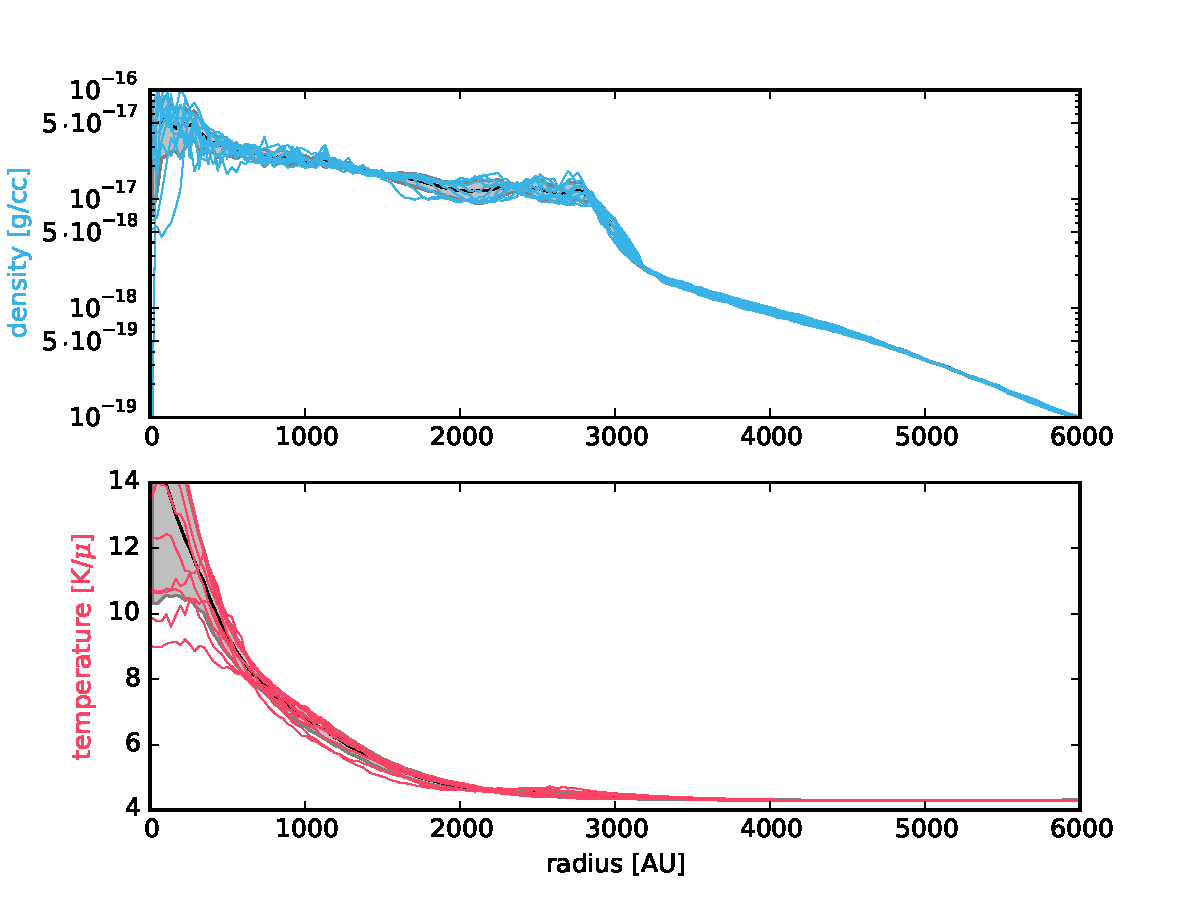
\includegraphics[width=0.99\textwidth]{Figures/var_rt_profiles/timeave_n1c01_6000AU}
 %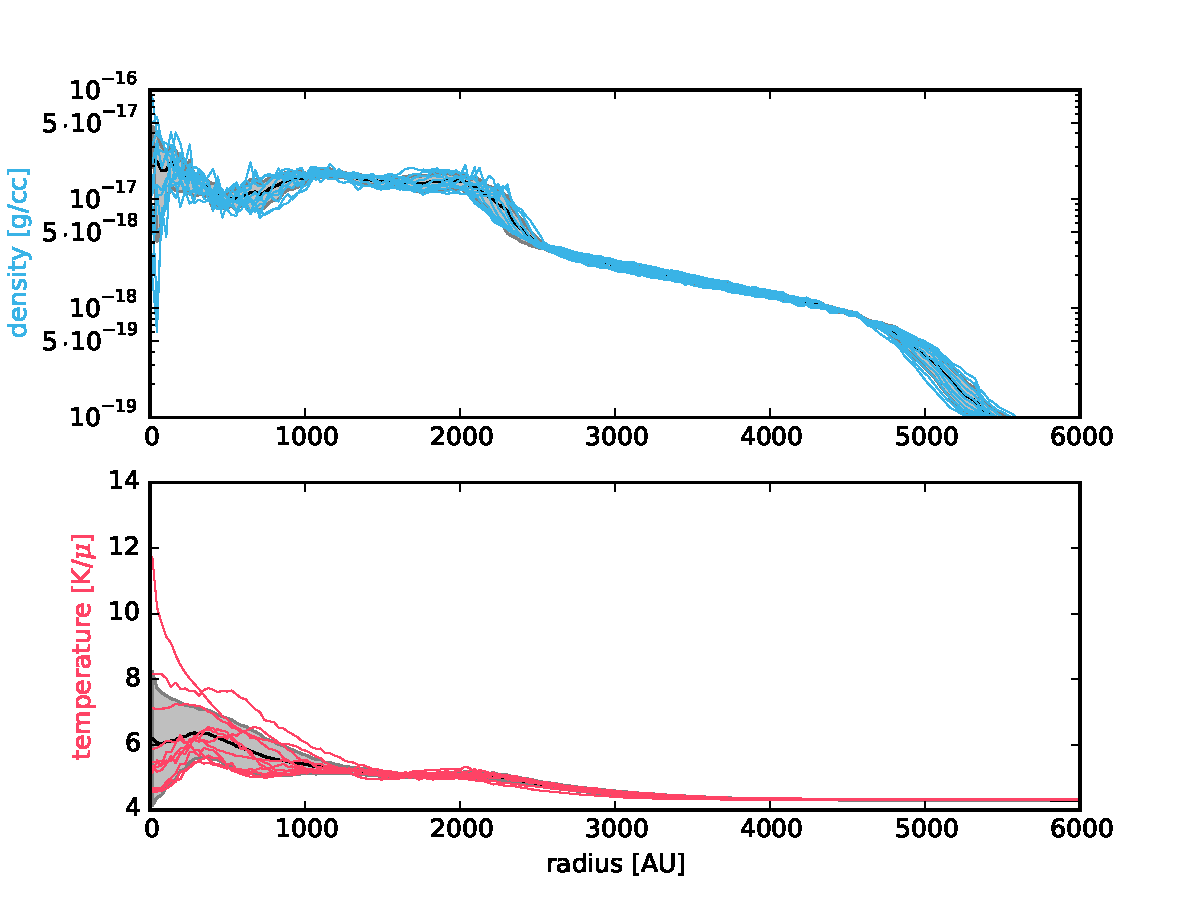
\includegraphics[width=0.99\textwidth]{Figures/var_rt_profiles/timeave_n1c1_6000AU}
 %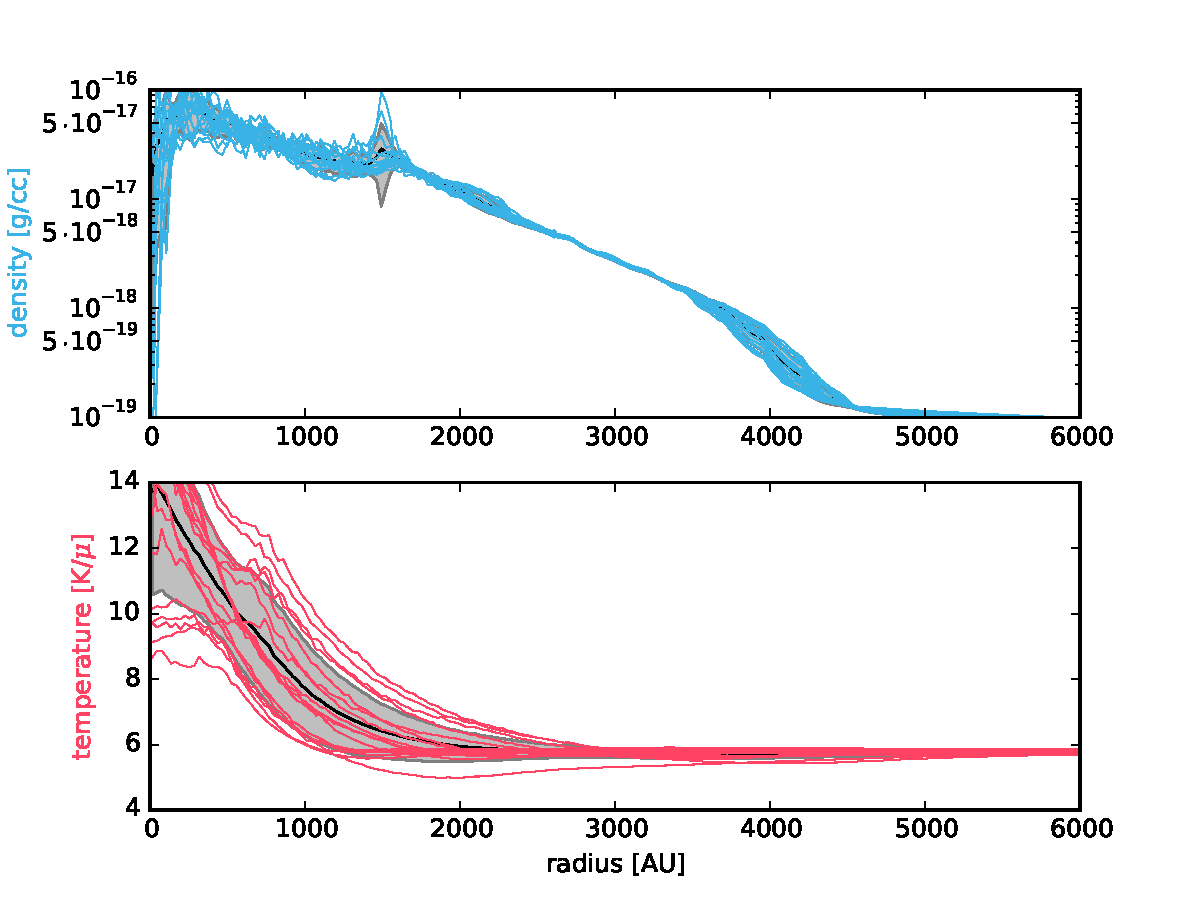
\includegraphics[width=0.99\textwidth]{Figures/var_rt_profiles/timeave_n1c10_6000AU_80_85kyrs}
 \captionsetup{justification=justified,singlelinecheck=false,width=\linewidth}
 \decoRule
 \caption[\code{nsub100c0.1} profiles]{Density and temperature profile of the \code{nsub100c0.1} run}
\label{fig:n100c0.1_profile}
\end{figure*}
\FloatBarrier

\begin{figure*}[!htb]
 \centering
 %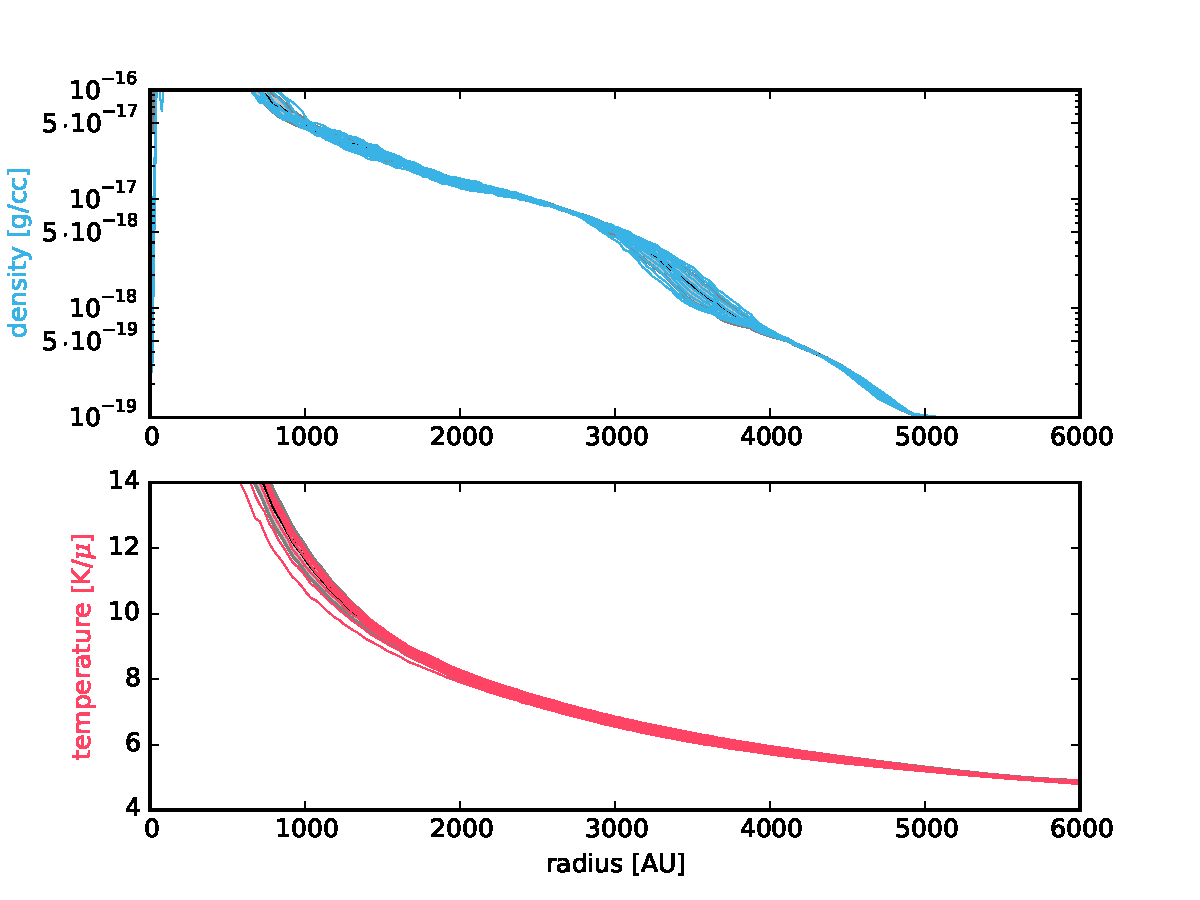
\includegraphics[width=0.99\textwidth]{Figures/var_rt_profiles/timeave_n100c01_6000AU}
 %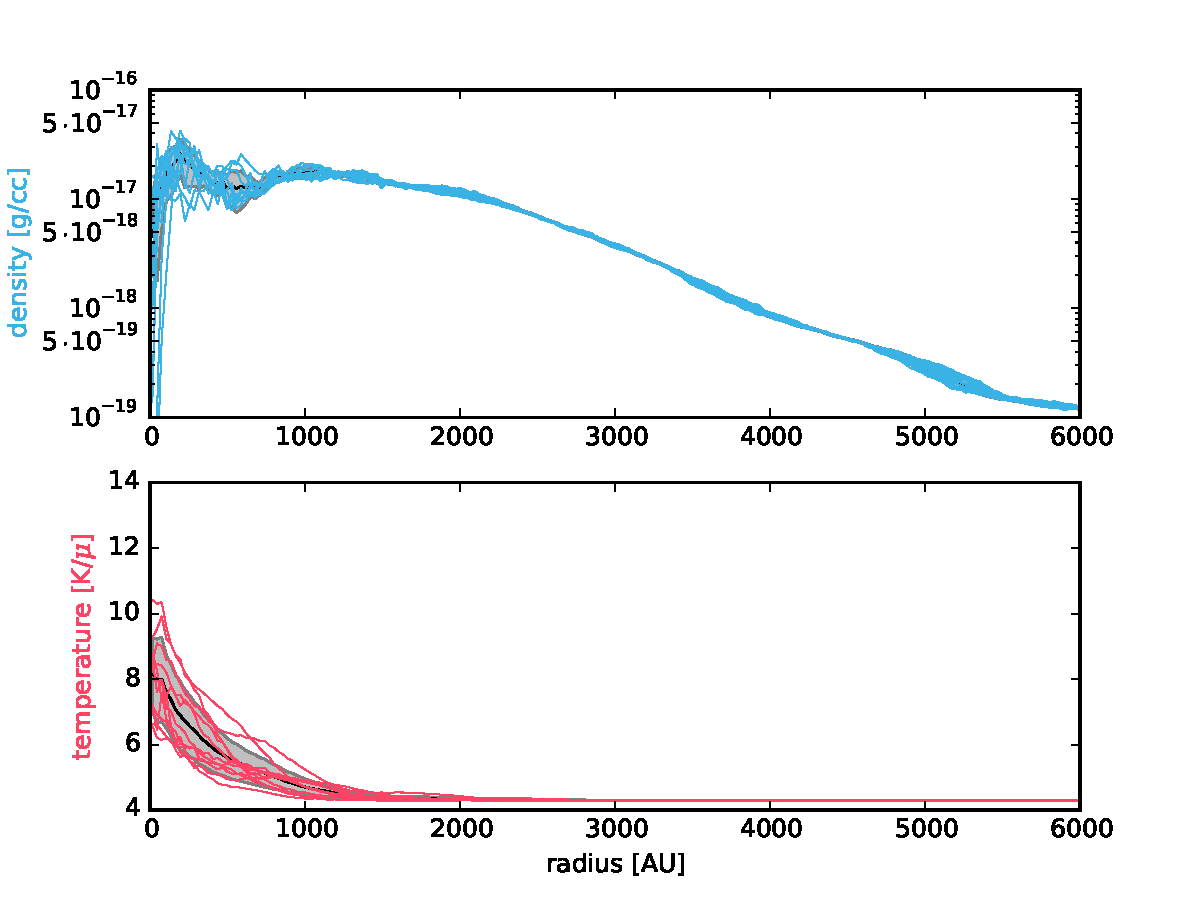
\includegraphics[width=0.99\textwidth]{Figures/var_rt_profiles/timeave_n100c1_6000AU}
 %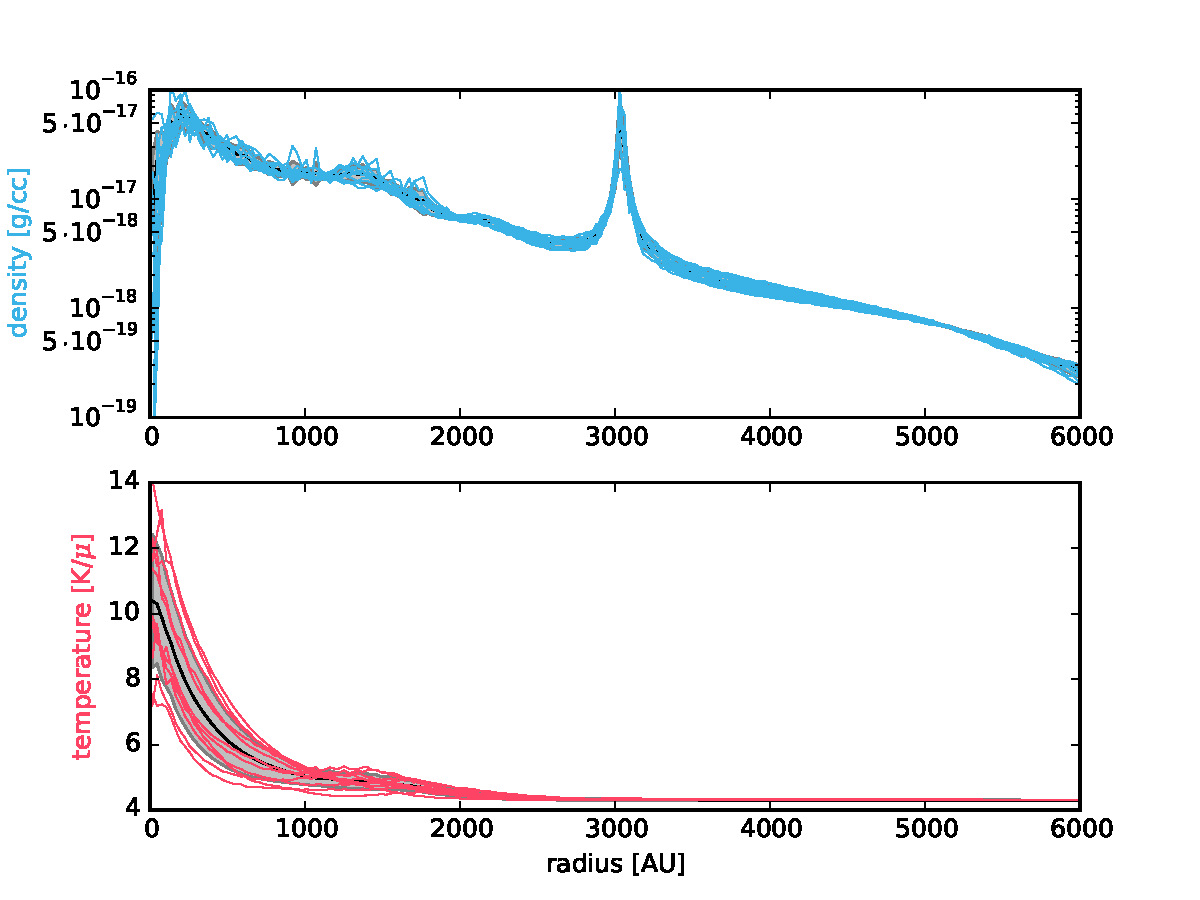
\includegraphics[width=0.99\textwidth]{Figures/var_rt_profiles/timeave_n100c10_6000AU}
 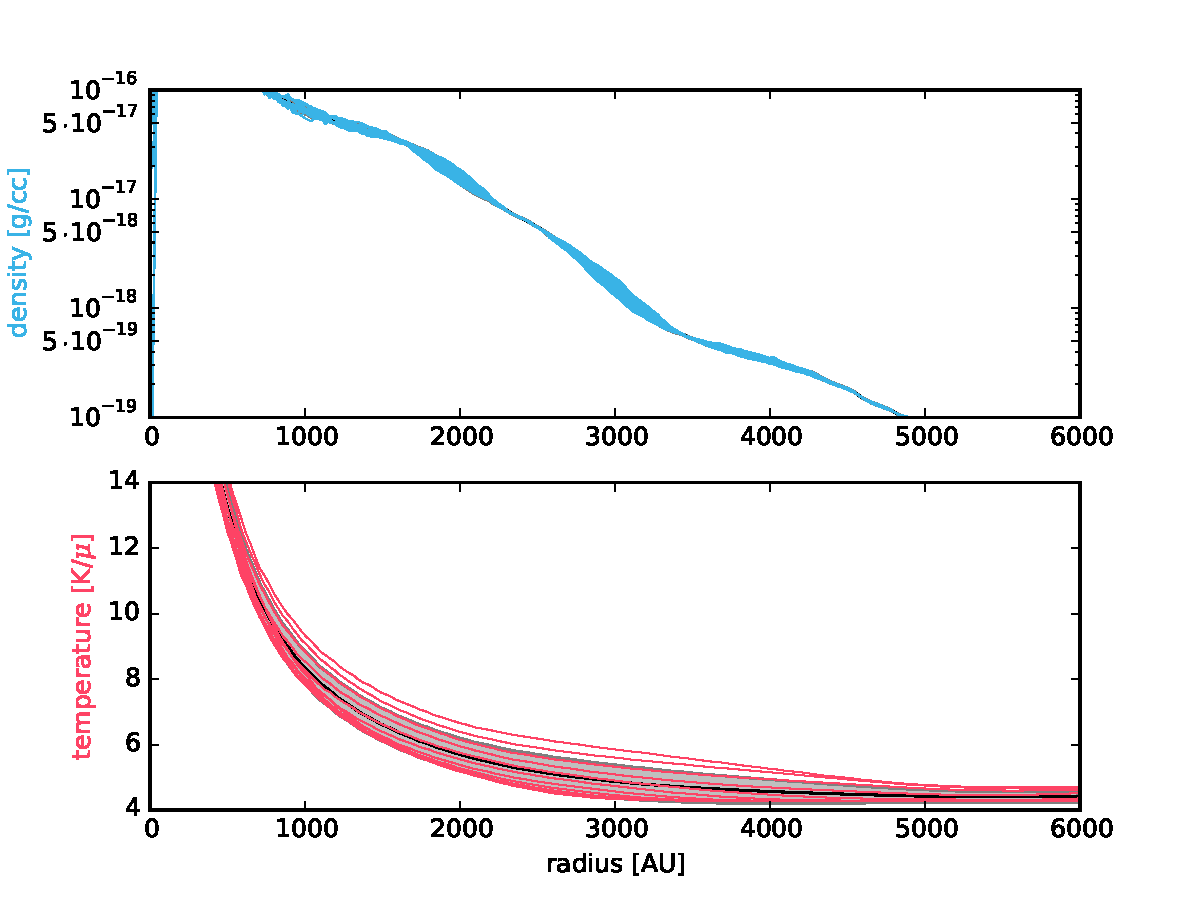
\includegraphics[width=0.99\textwidth]{Figures/var_rt_profiles/timeave_n10c01_6000AU}
 %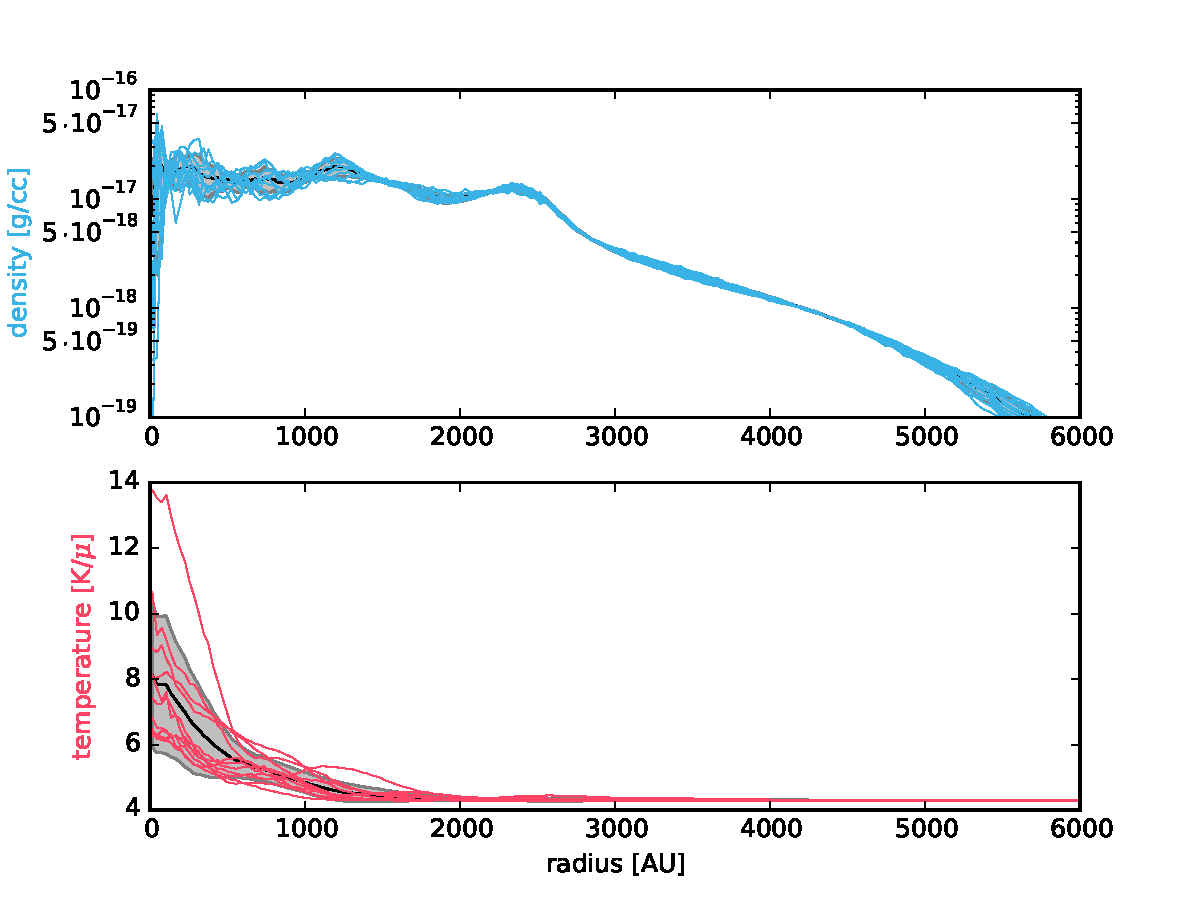
\includegraphics[width=0.99\textwidth]{Figures/var_rt_profiles/timeave_n10c1_6000AU}
 %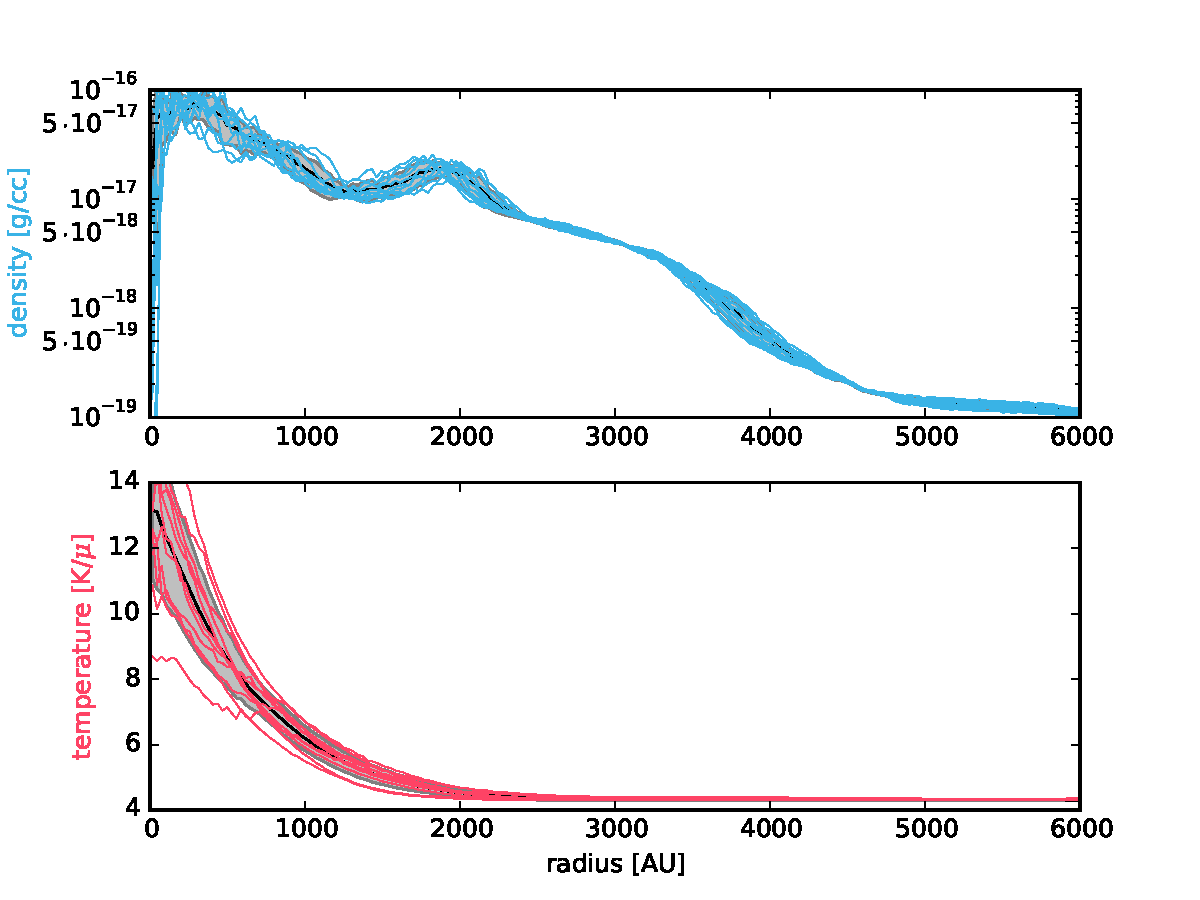
\includegraphics[width=0.99\textwidth]{Figures/var_rt_profiles/timeave_n10c10_6000AU}
 %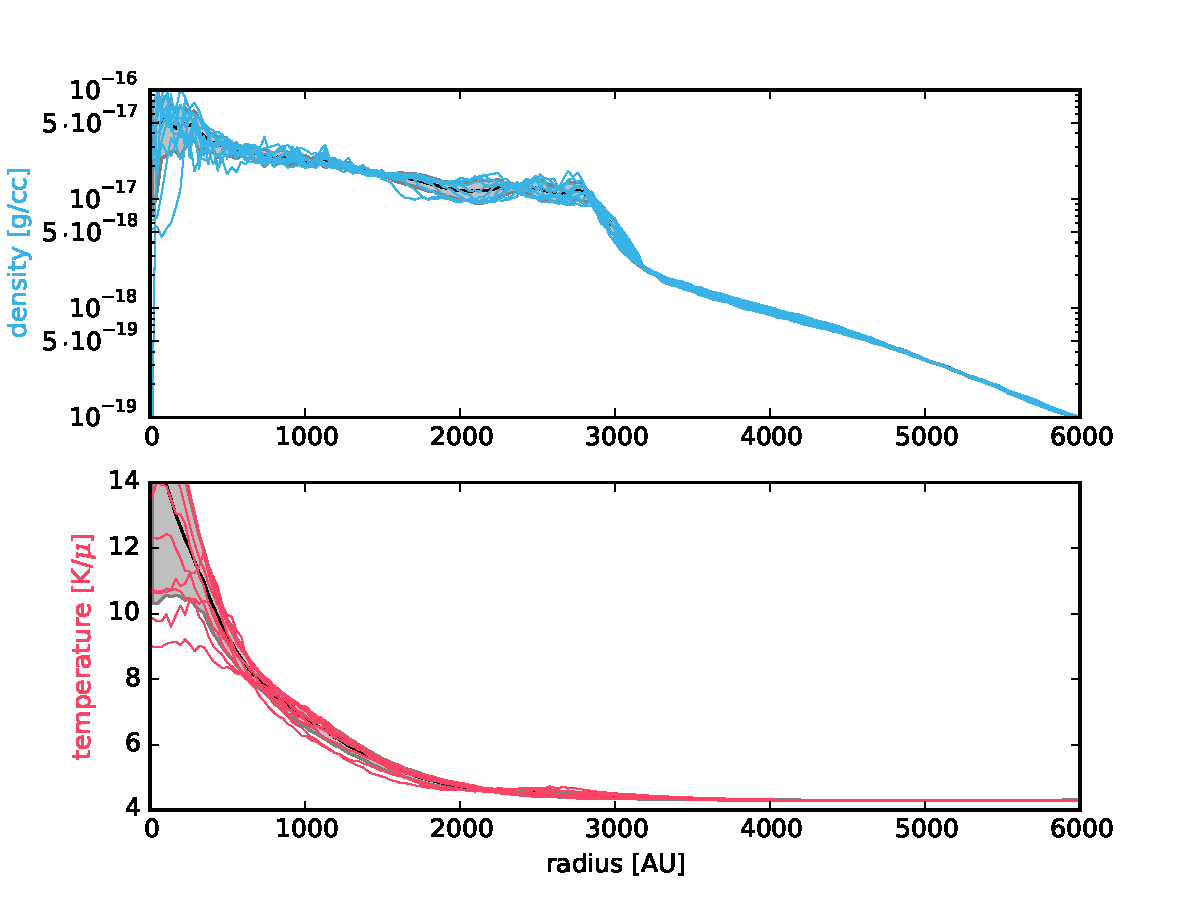
\includegraphics[width=0.99\textwidth]{Figures/var_rt_profiles/timeave_n1c01_6000AU}
 %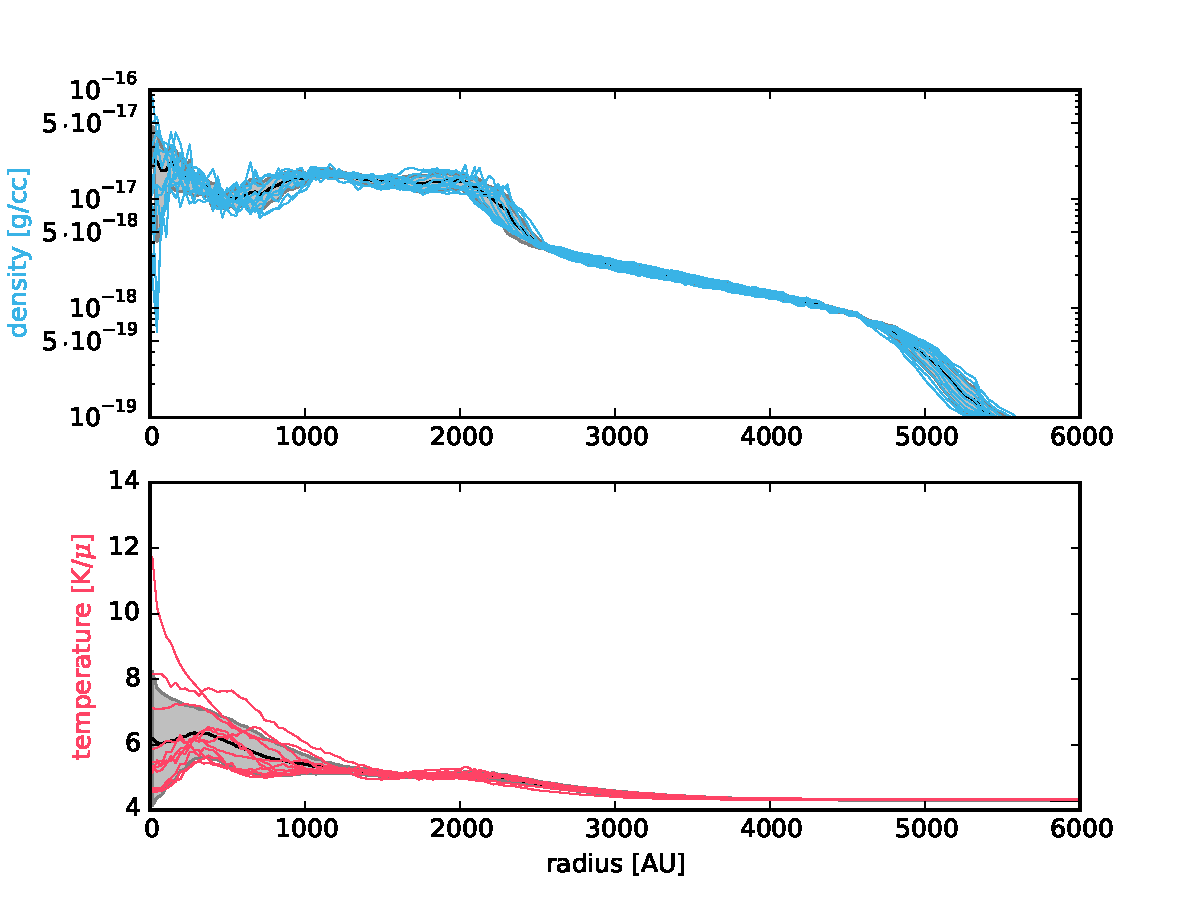
\includegraphics[width=0.99\textwidth]{Figures/var_rt_profiles/timeave_n1c1_6000AU}
 %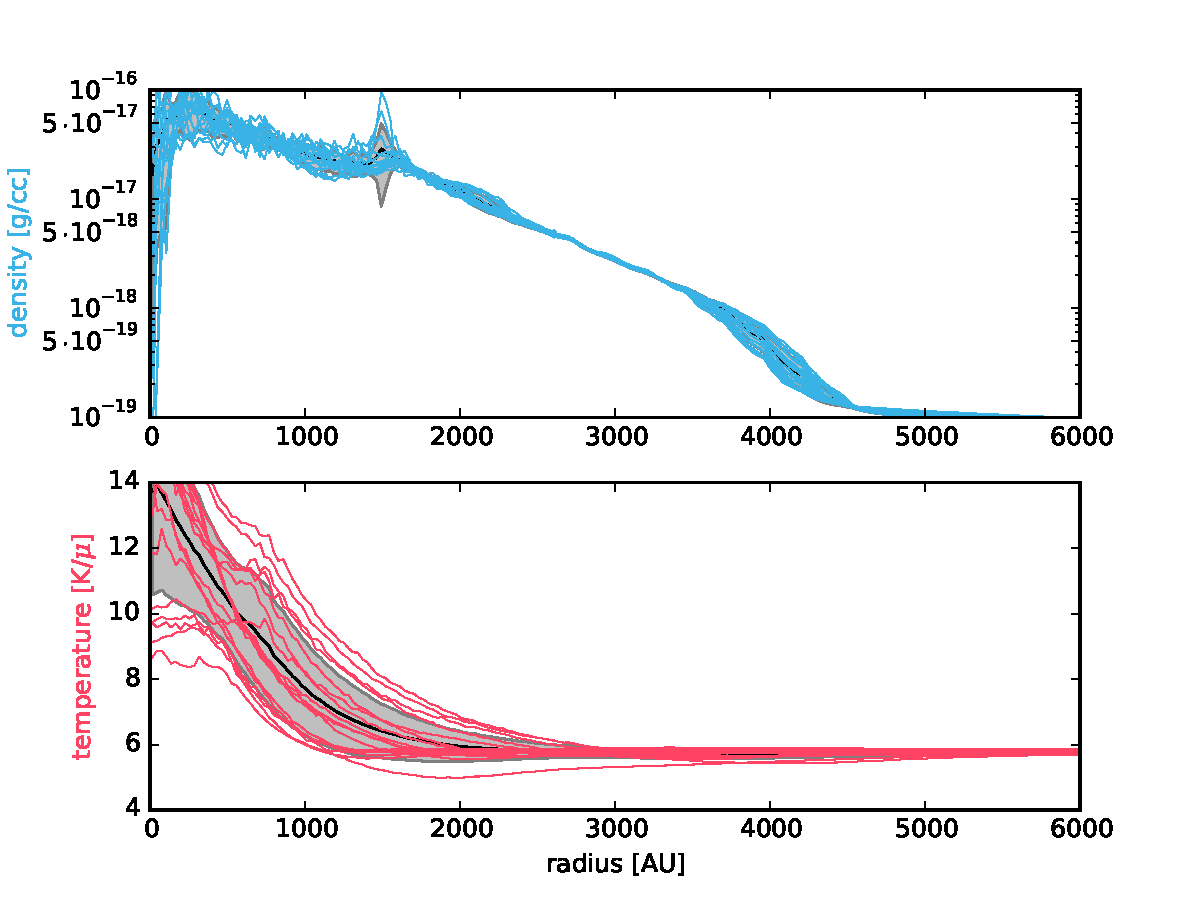
\includegraphics[width=0.99\textwidth]{Figures/var_rt_profiles/timeave_n1c10_6000AU_80_85kyrs}
 \captionsetup{justification=justified,singlelinecheck=false,width=\linewidth}
 \decoRule
 \caption[\code{nsub010c0.1} profiles]{Density and temperature profile of the \code{nsub010c0.1} run}
\label{fig:n10c0.1_profile}
\end{figure*}
\FloatBarrier

\begin{figure*}[!htb]
 \centering
 %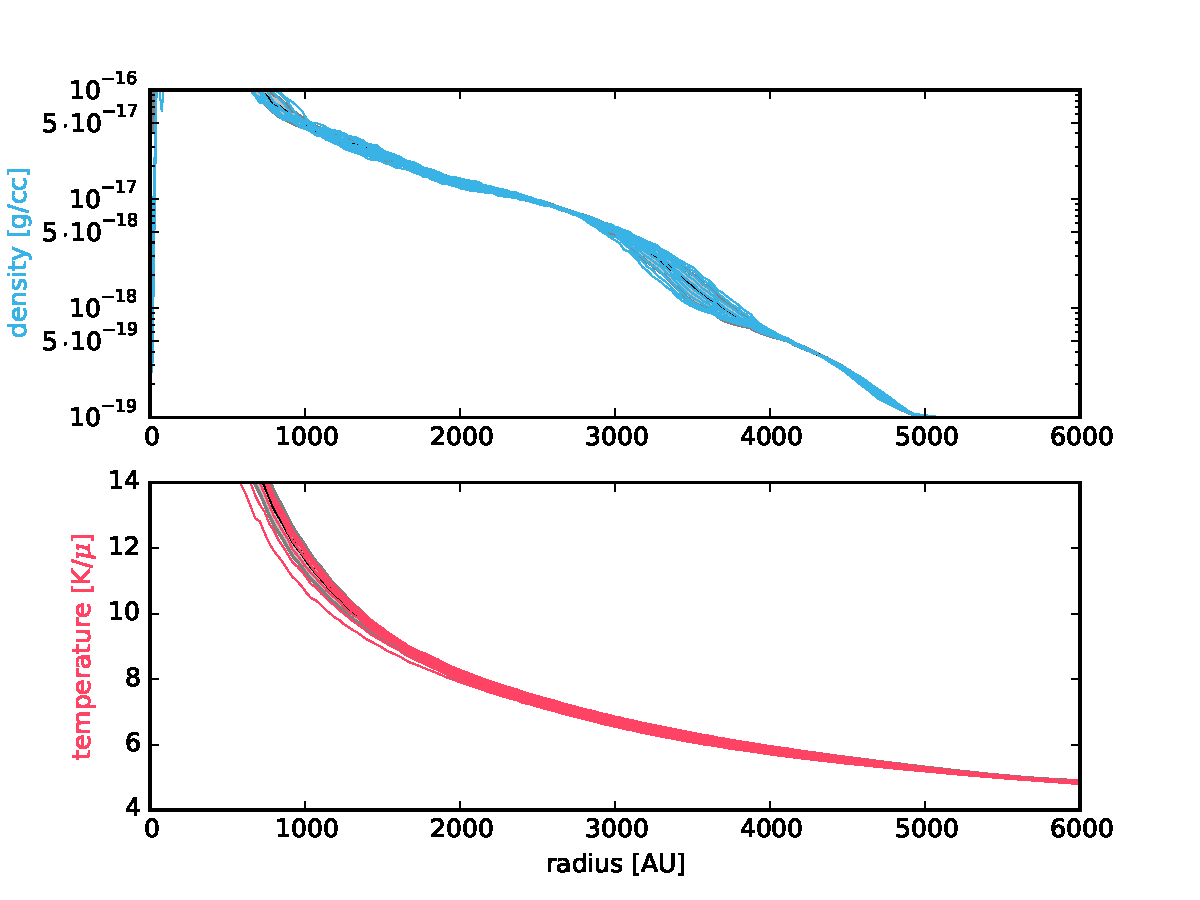
\includegraphics[width=0.99\textwidth]{Figures/var_rt_profiles/timeave_n100c01_6000AU}
 %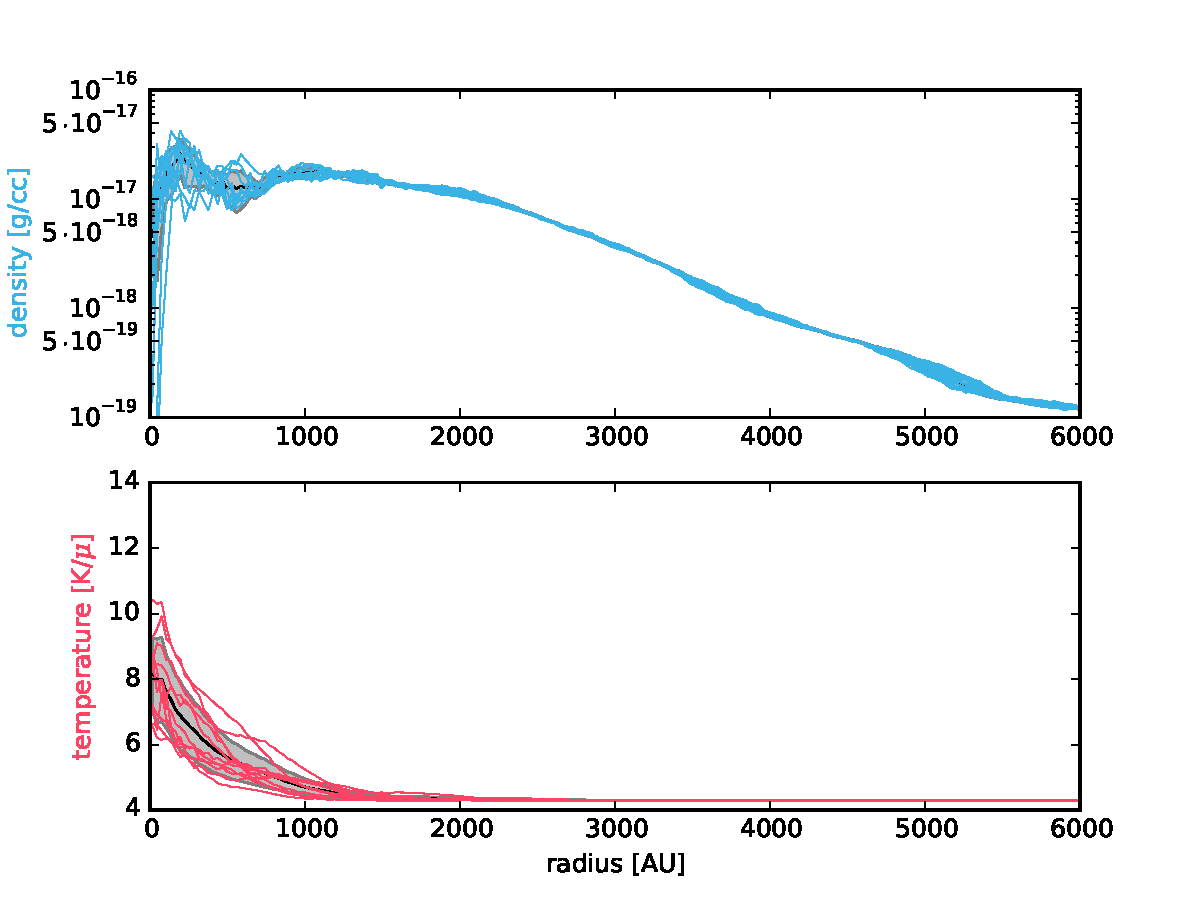
\includegraphics[width=0.99\textwidth]{Figures/var_rt_profiles/timeave_n100c1_6000AU}
 %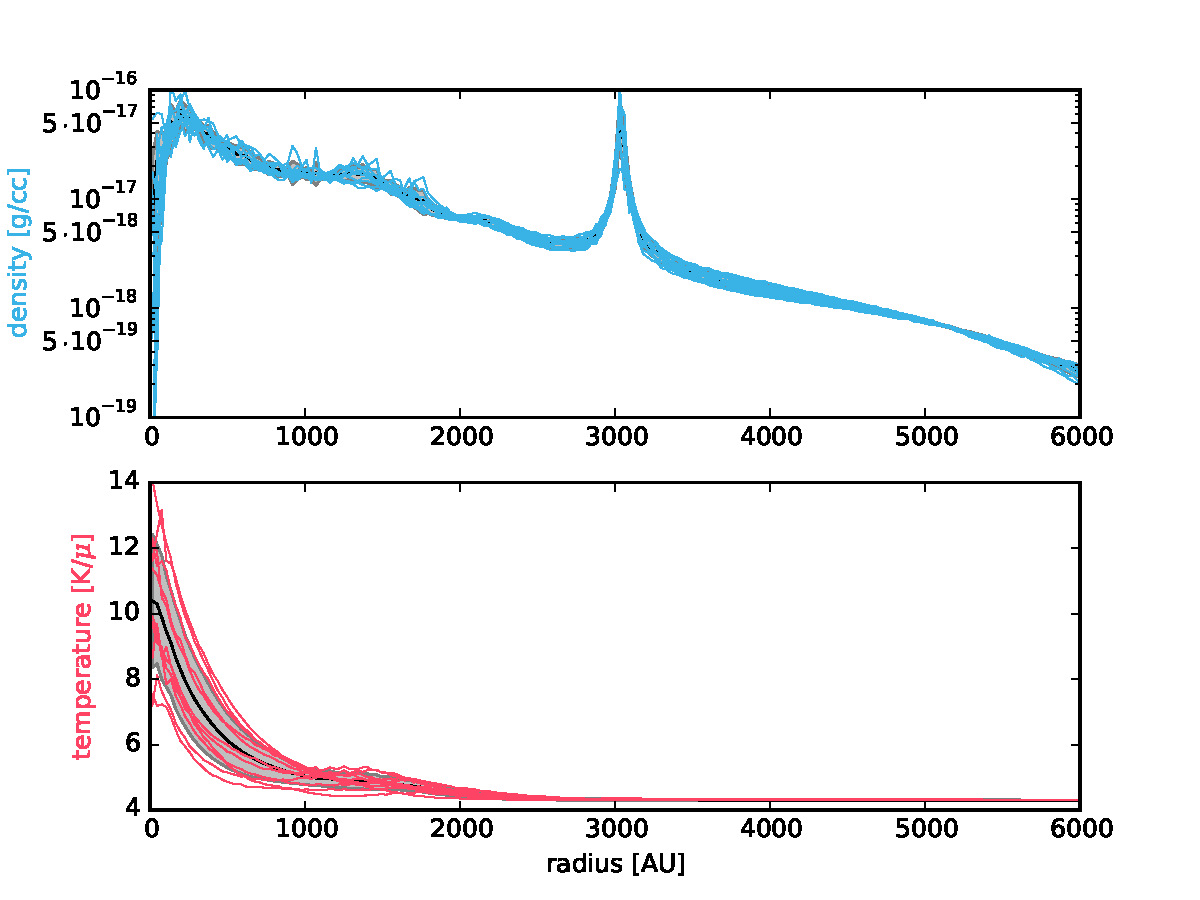
\includegraphics[width=0.99\textwidth]{Figures/var_rt_profiles/timeave_n100c10_6000AU}
 %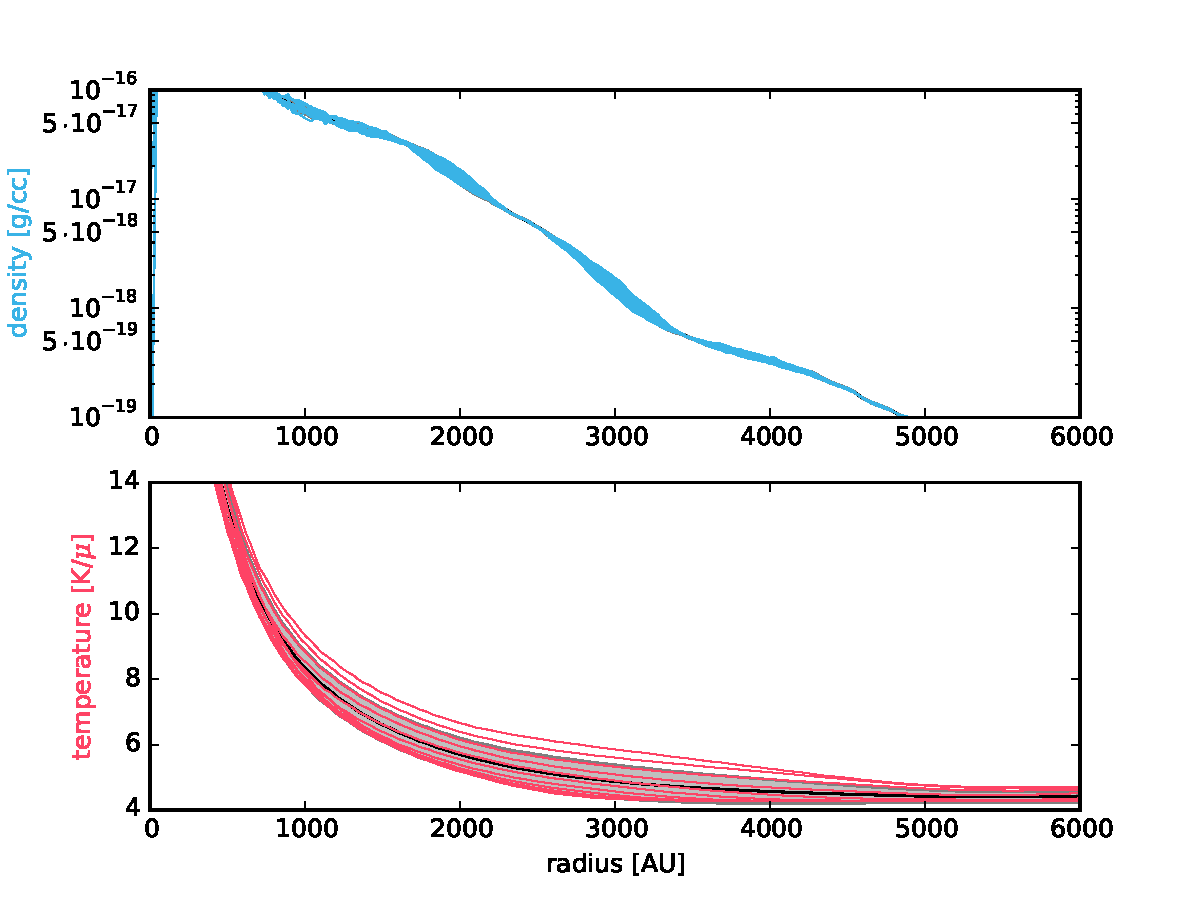
\includegraphics[width=0.99\textwidth]{Figures/var_rt_profiles/timeave_n10c01_6000AU}
 %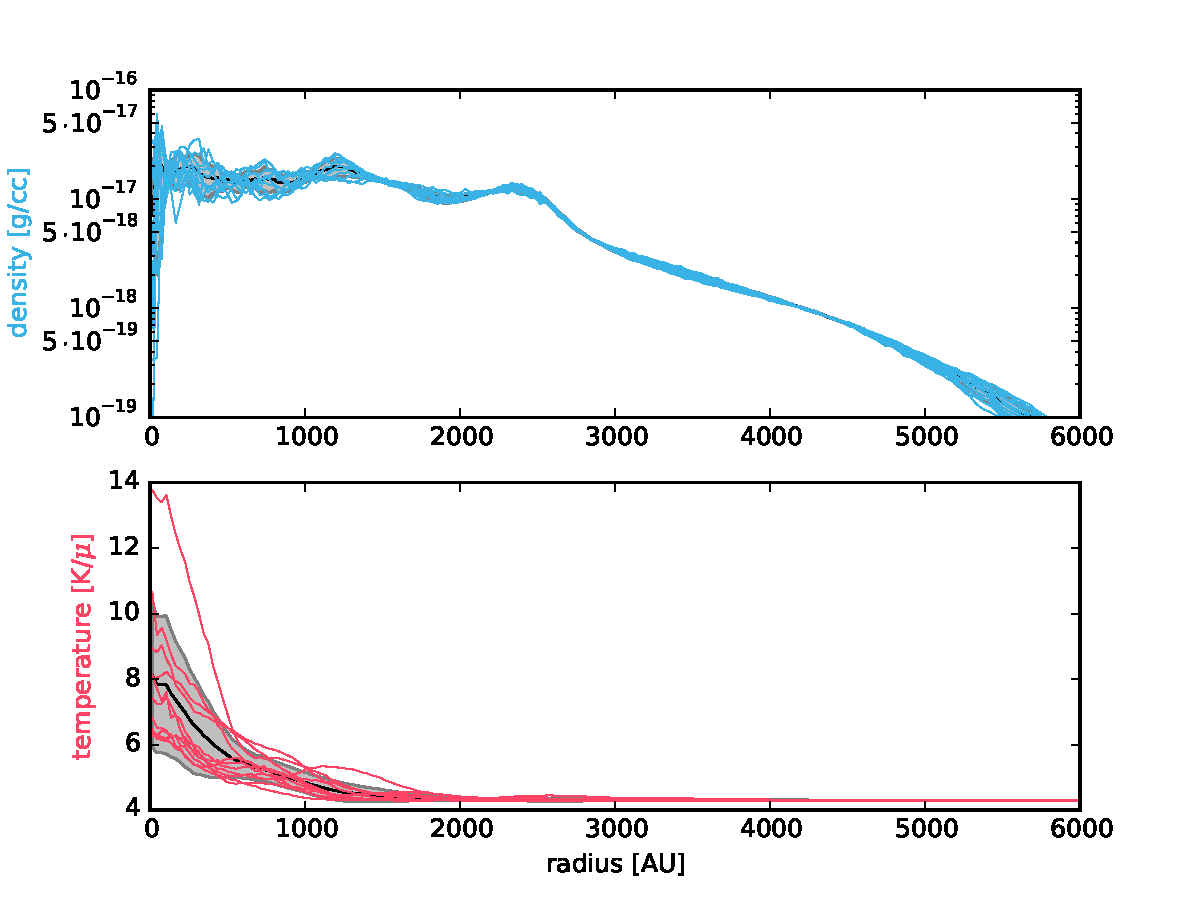
\includegraphics[width=0.99\textwidth]{Figures/var_rt_profiles/timeave_n10c1_6000AU}
 %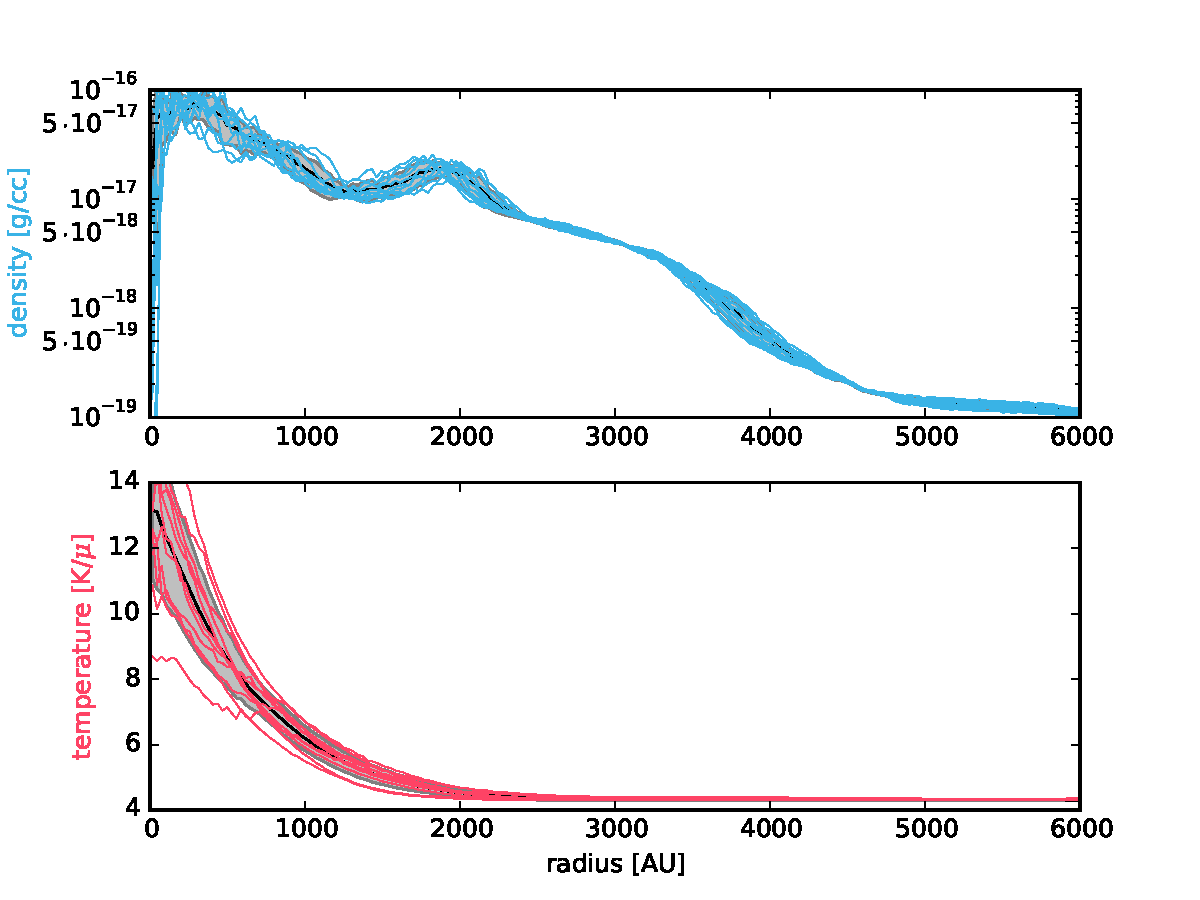
\includegraphics[width=0.99\textwidth]{Figures/var_rt_profiles/timeave_n10c10_6000AU}
 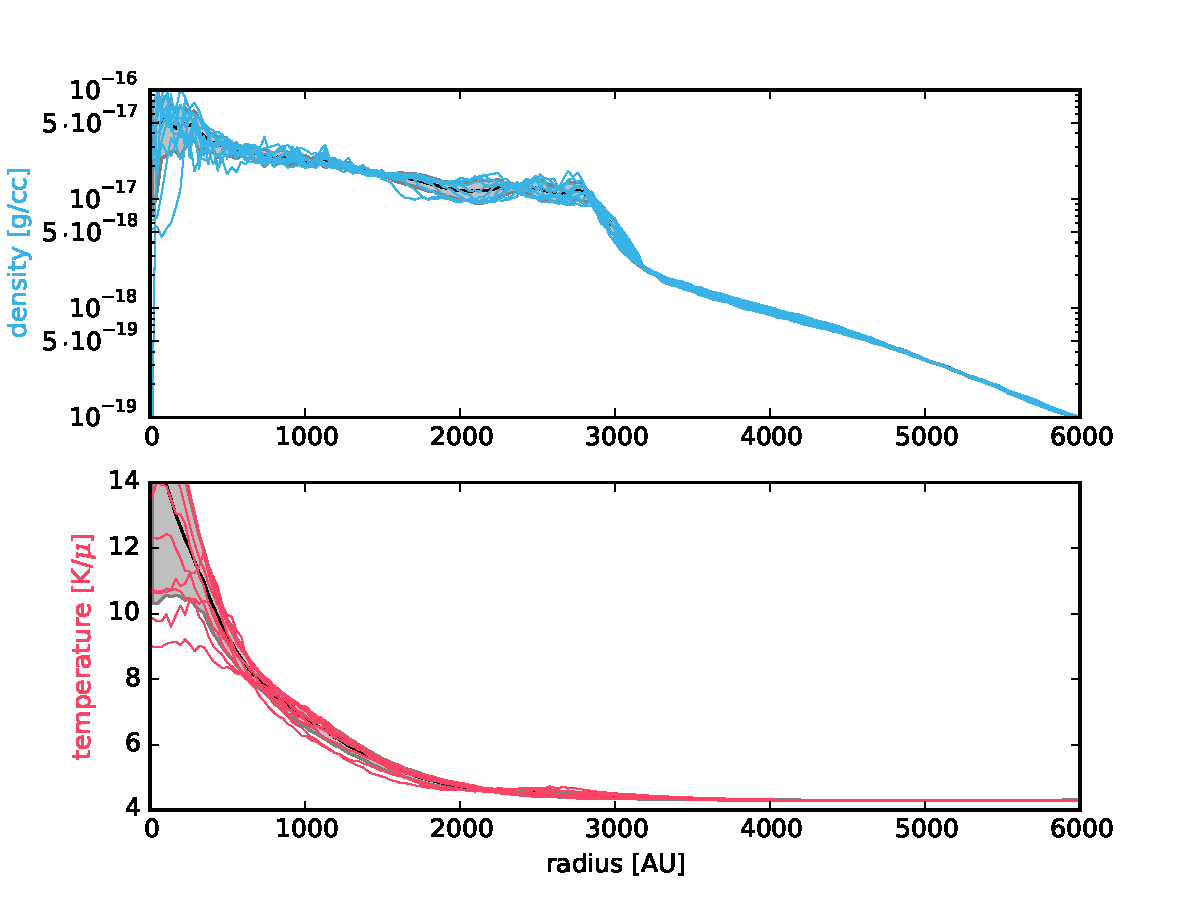
\includegraphics[width=0.99\textwidth]{Figures/var_rt_profiles/timeave_n1c01_6000AU}
 %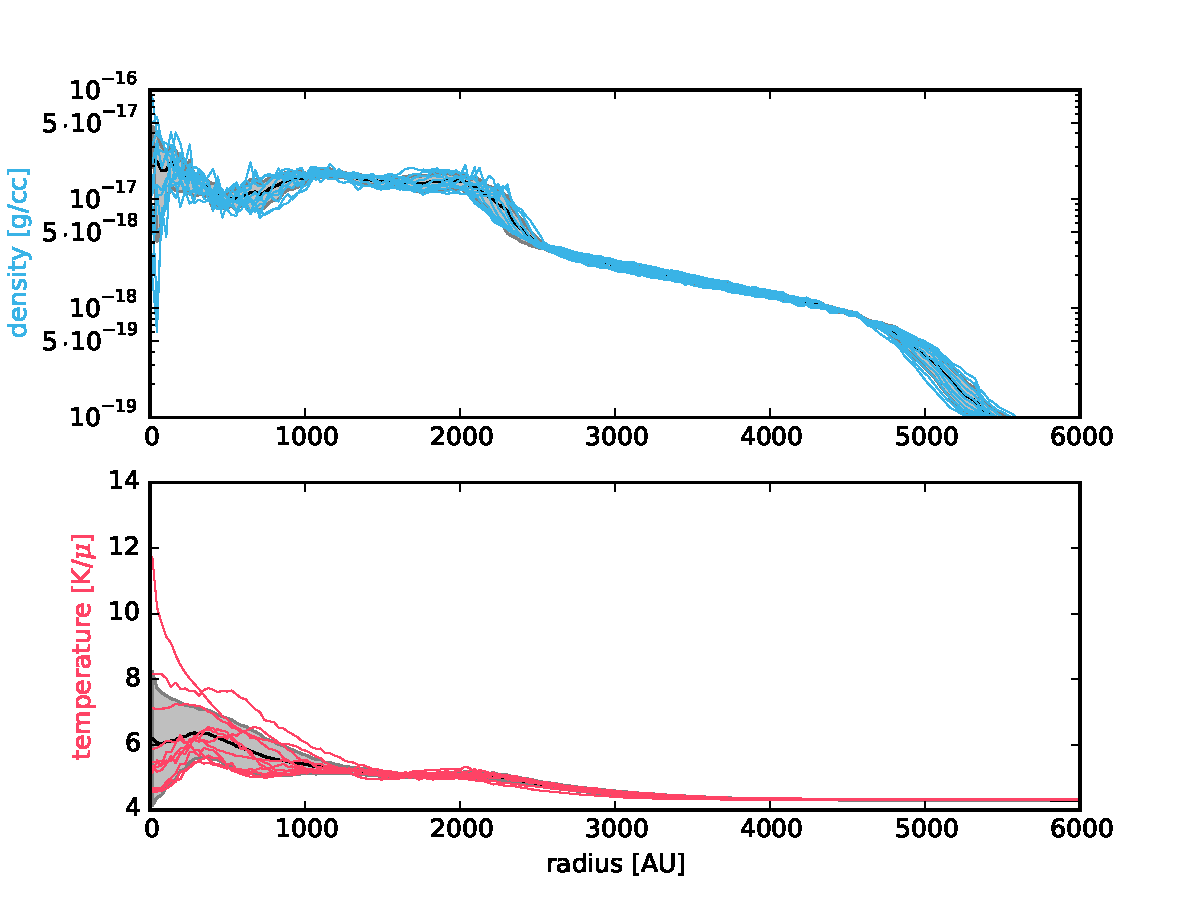
\includegraphics[width=0.99\textwidth]{Figures/var_rt_profiles/timeave_n1c1_6000AU}
 %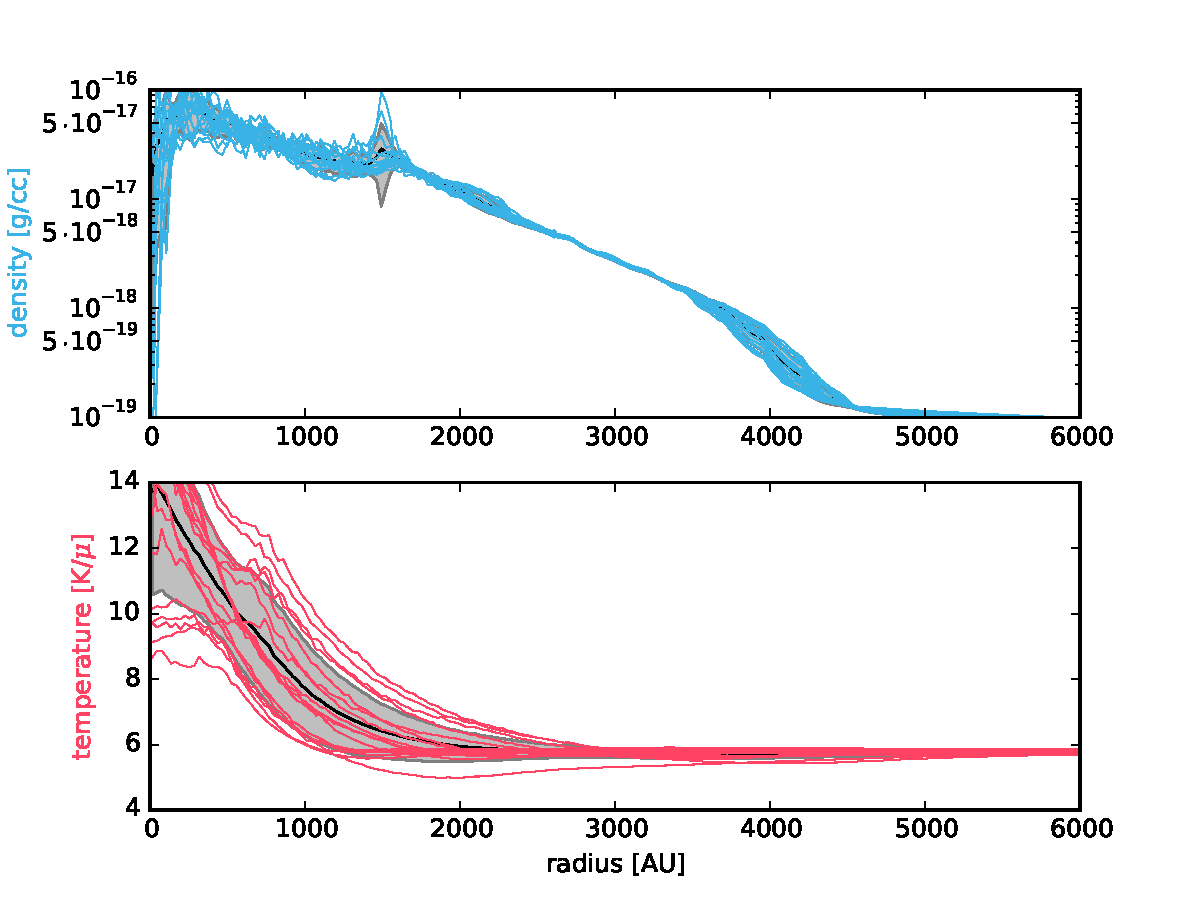
\includegraphics[width=0.99\textwidth]{Figures/var_rt_profiles/timeave_n1c10_6000AU_80_85kyrs}
 \captionsetup{justification=justified,singlelinecheck=false,width=\linewidth}
 \decoRule
 \caption[\code{nsub001c0.1} profiles]{Density and temperature profile of the \code{nsub001c0.1} run}
\label{fig:n1c0.1_profile}
\end{figure*}
\FloatBarrier

% 1.0 c_frac_speed_factor

\begin{figure*}[!htb]
 \centering
 %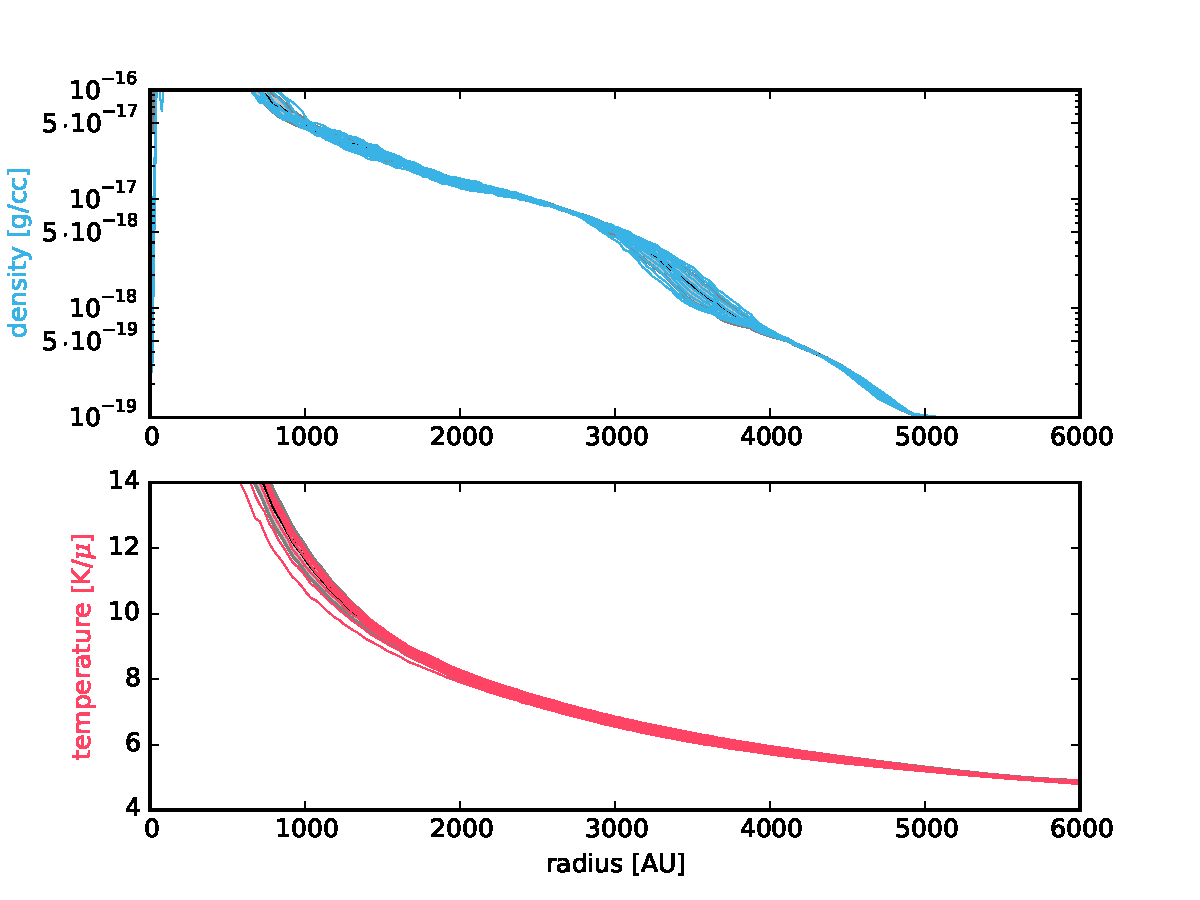
\includegraphics[width=0.99\textwidth]{Figures/var_rt_profiles/timeave_n100c01_6000AU}
 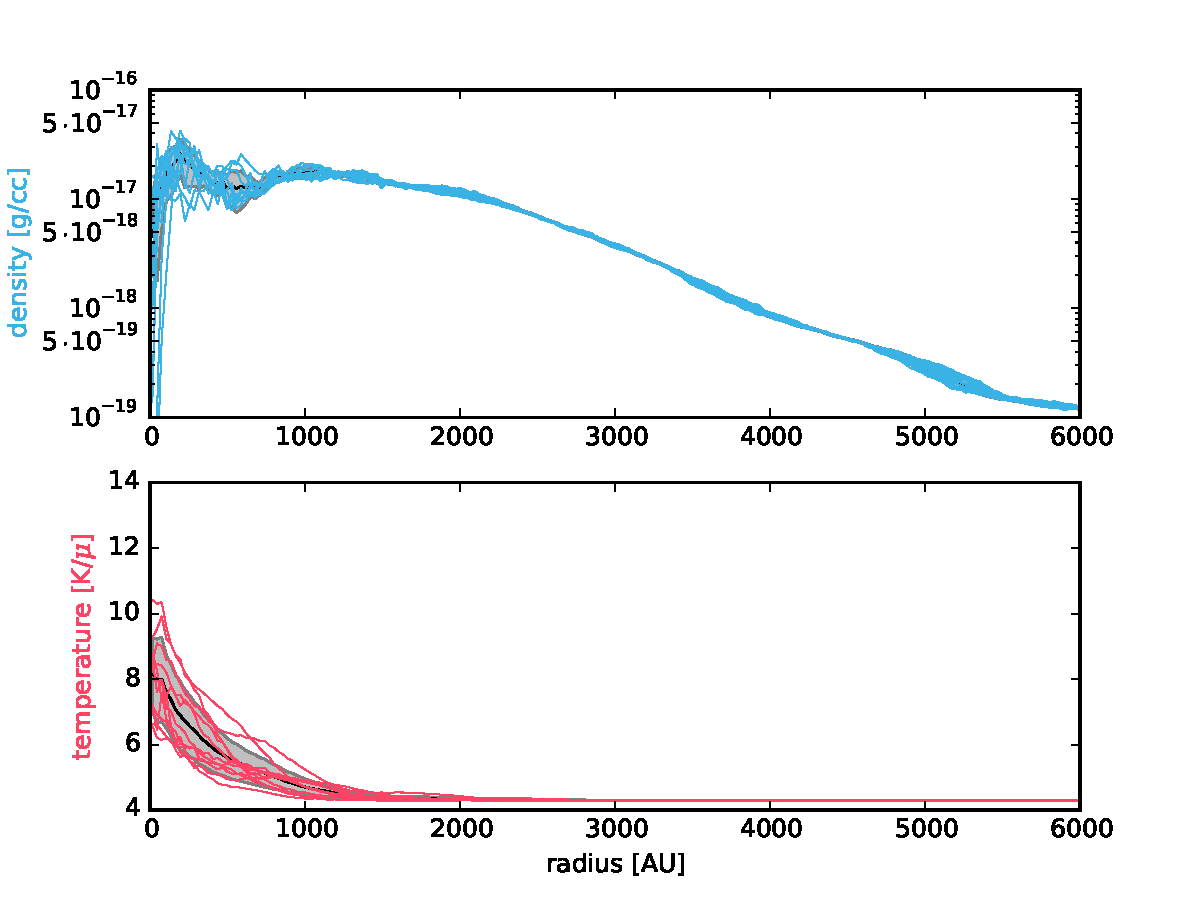
\includegraphics[width=0.99\textwidth]{Figures/var_rt_profiles/timeave_n100c1_6000AU}
 %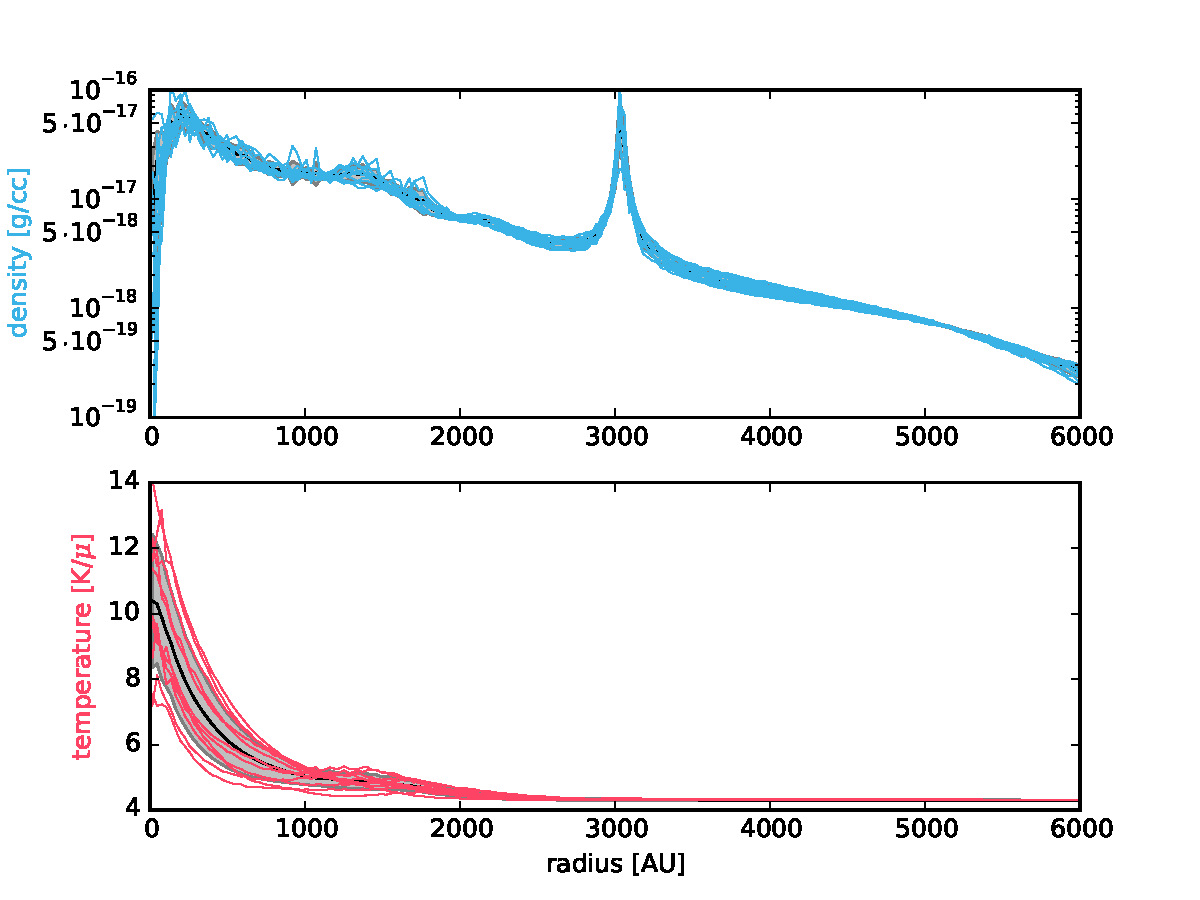
\includegraphics[width=0.99\textwidth]{Figures/var_rt_profiles/timeave_n100c10_6000AU}
 %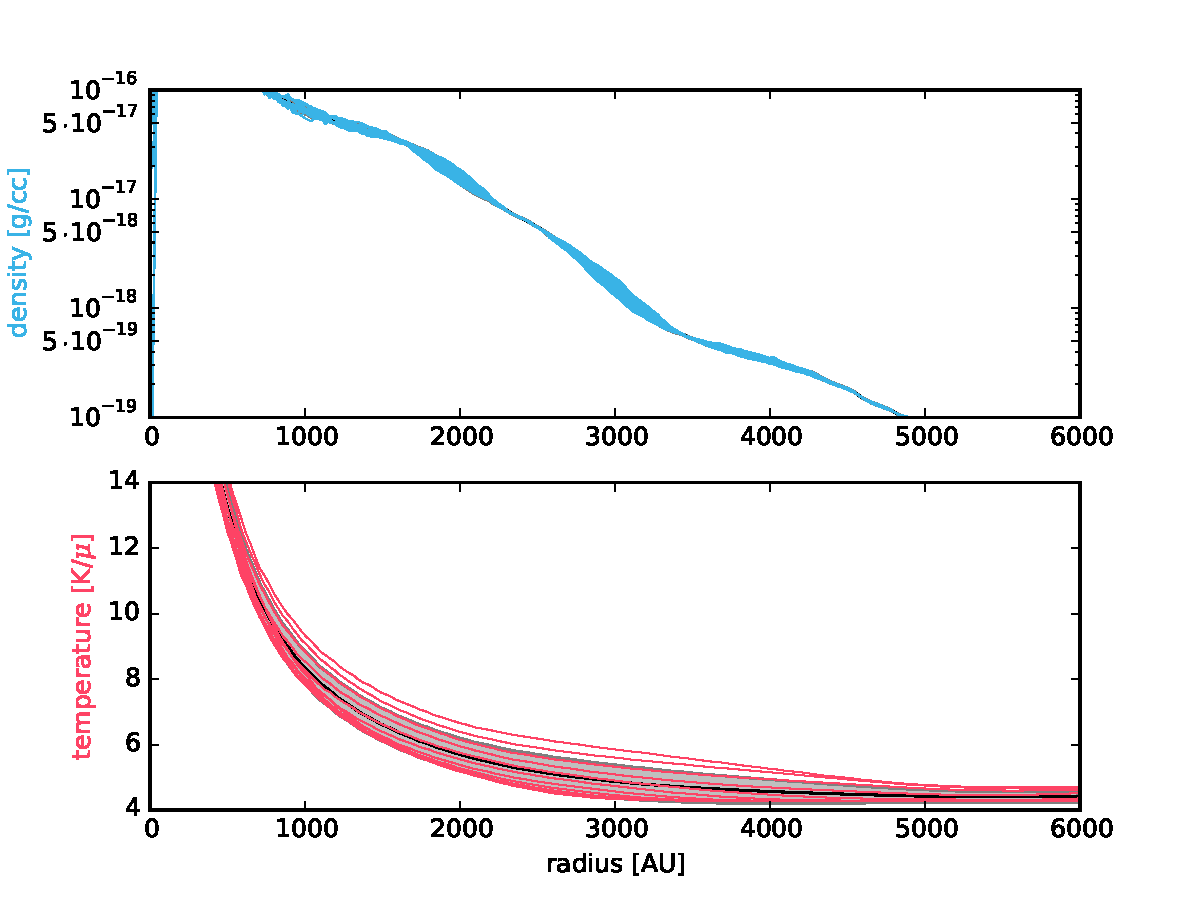
\includegraphics[width=0.99\textwidth]{Figures/var_rt_profiles/timeave_n10c01_6000AU}
 %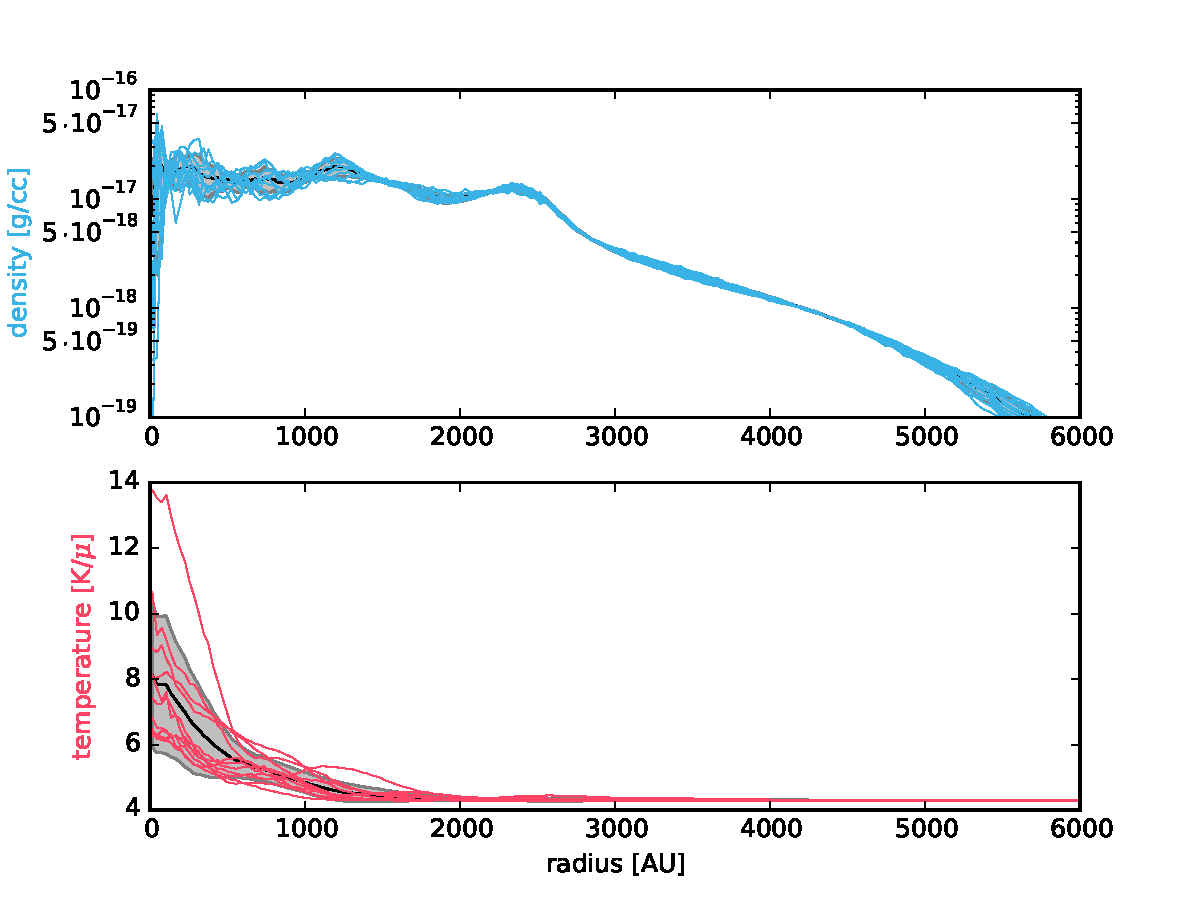
\includegraphics[width=0.99\textwidth]{Figures/var_rt_profiles/timeave_n10c1_6000AU}
 %\includegraphics[width=0.99\textwidth]{Figures/var_rt_profiles/timeave_n10c10_6000AU}
 %\includegraphics[width=0.99\textwidth]{Figures/var_rt_profiles/timeave_n1c01_6000AU}
 %\includegraphics[width=0.99\textwidth]{Figures/var_rt_profiles/timeave_n1c1_6000AU}
 %\includegraphics[width=0.99\textwidth]{Figures/var_rt_profiles/timeave_n1c10_6000AU_80_85kyrs}
 \captionsetup{justification=justified,singlelinecheck=false,width=\linewidth}
 \decoRule
 \caption[\code{nsub100c1} profiles]{Density and temperature profile of the \code{nsub100c1} run}
\label{fig:n100c1.0_profile}
\end{figure*}
\FloatBarrier

\begin{figure*}[!htb]
 \centering
 %\includegraphics[width=0.99\textwidth]{Figures/var_rt_profiles/timeave_n100c01_6000AU}
 %\includegraphics[width=0.99\textwidth]{Figures/var_rt_profiles/timeave_n100c1_6000AU}
 %\includegraphics[width=0.99\textwidth]{Figures/var_rt_profiles/timeave_n100c10_6000AU}
 %\includegraphics[width=0.99\textwidth]{Figures/var_rt_profiles/timeave_n10c01_6000AU}
 \includegraphics[width=0.99\textwidth]{Figures/var_rt_profiles/timeave_n10c1_6000AU}
 %\includegraphics[width=0.99\textwidth]{Figures/var_rt_profiles/timeave_n10c10_6000AU}
 %\includegraphics[width=0.99\textwidth]{Figures/var_rt_profiles/timeave_n1c01_6000AU}
 %\includegraphics[width=0.99\textwidth]{Figures/var_rt_profiles/timeave_n1c1_6000AU}
 %\includegraphics[width=0.99\textwidth]{Figures/var_rt_profiles/timeave_n1c10_6000AU_80_85kyrs}
 \captionsetup{justification=justified,singlelinecheck=false,width=\linewidth}
 \decoRule
 \caption[\code{nsub010c1} profiles]{Density and temperature profile of the \code{nsub010c1} run}
\label{fig:n10c1.0_profile}
\end{figure*}
\FloatBarrier

\begin{figure*}[!htb]
 \centering
 %\includegraphics[width=0.99\textwidth]{Figures/var_rt_profiles/timeave_n100c01_6000AU}
 %\includegraphics[width=0.99\textwidth]{Figures/var_rt_profiles/timeave_n100c1_6000AU}
 %\includegraphics[width=0.99\textwidth]{Figures/var_rt_profiles/timeave_n100c10_6000AU}
 %\includegraphics[width=0.99\textwidth]{Figures/var_rt_profiles/timeave_n10c01_6000AU}
 %\includegraphics[width=0.99\textwidth]{Figures/var_rt_profiles/timeave_n10c1_6000AU}
 %\includegraphics[width=0.99\textwidth]{Figures/var_rt_profiles/timeave_n10c10_6000AU}
 %\includegraphics[width=0.99\textwidth]{Figures/var_rt_profiles/timeave_n1c01_6000AU}
 \includegraphics[width=0.99\textwidth]{Figures/var_rt_profiles/timeave_n1c1_6000AU}
 %\includegraphics[width=0.99\textwidth]{Figures/var_rt_profiles/timeave_n1c10_6000AU_80_85kyrs}
 \captionsetup{justification=justified,singlelinecheck=false,width=\linewidth}
 \decoRule
 \caption[\code{nsub001c1} profiles]{Density and temperature profile of the \code{nsub001c1} run}
\label{fig:n1c1.0_profile}
\end{figure*}
\FloatBarrier

% 10. c_frac_speed_factor

\begin{figure*}[!htb]
 \centering
 %\includegraphics[width=0.99\textwidth]{Figures/var_rt_profiles/timeave_n100c01_6000AU}
 %\includegraphics[width=0.99\textwidth]{Figures/var_rt_profiles/timeave_n100c1_6000AU}
 \includegraphics[width=0.99\textwidth]{Figures/var_rt_profiles/timeave_n100c10_6000AU}
 %\includegraphics[width=0.99\textwidth]{Figures/var_rt_profiles/timeave_n10c01_6000AU}
 %\includegraphics[width=0.99\textwidth]{Figures/var_rt_profiles/timeave_n10c1_6000AU}
 %\includegraphics[width=0.99\textwidth]{Figures/var_rt_profiles/timeave_n10c10_6000AU}
 %\includegraphics[width=0.99\textwidth]{Figures/var_rt_profiles/timeave_n1c01_6000AU}
 %\includegraphics[width=0.99\textwidth]{Figures/var_rt_profiles/timeave_n1c1_6000AU}
 %\includegraphics[width=0.99\textwidth]{Figures/var_rt_profiles/timeave_n1c10_6000AU_80_85kyrs}
 \captionsetup{justification=justified,singlelinecheck=false,width=\linewidth}
 \decoRule
 \caption[\code{nsub100c10} profiles]{Density and temperature profile of the \code{nsub100c10} run}
\label{fig:n100c10.0_profile}
\end{figure*}
\FloatBarrier


\begin{figure*}[!htb]
 \centering
 %\includegraphics[width=0.99\textwidth]{Figures/var_rt_profiles/timeave_n100c01_6000AU}
 %\includegraphics[width=0.99\textwidth]{Figures/var_rt_profiles/timeave_n100c1_6000AU}
 %\includegraphics[width=0.99\textwidth]{Figures/var_rt_profiles/timeave_n100c10_6000AU}
 %\includegraphics[width=0.99\textwidth]{Figures/var_rt_profiles/timeave_n10c01_6000AU}
 %\includegraphics[width=0.99\textwidth]{Figures/var_rt_profiles/timeave_n10c1_6000AU}
 \includegraphics[width=0.99\textwidth]{Figures/var_rt_profiles/timeave_n10c10_6000AU}
 %\includegraphics[width=0.99\textwidth]{Figures/var_rt_profiles/timeave_n1c01_6000AU}
 %\includegraphics[width=0.99\textwidth]{Figures/var_rt_profiles/timeave_n1c1_6000AU}
 %\includegraphics[width=0.99\textwidth]{Figures/var_rt_profiles/timeave_n1c10_6000AU_80_85kyrs}
 \captionsetup{justification=justified,singlelinecheck=false,width=\linewidth}
 \decoRule
 \caption[\code{nsub010c10} profiles]{Density and temperature profile of the \code{nsub010c10} run}
\label{fig:n10c10.0_profile}
\end{figure*}
\FloatBarrier

\begin{figure*}[!htb]
 \centering
 %\includegraphics[width=0.99\textwidth]{Figures/var_rt_profiles/timeave_n100c01_6000AU}
 %\includegraphics[width=0.99\textwidth]{Figures/var_rt_profiles/timeave_n100c1_6000AU}
 %\includegraphics[width=0.99\textwidth]{Figures/var_rt_profiles/timeave_n100c10_6000AU}
 %\includegraphics[width=0.99\textwidth]{Figures/var_rt_profiles/timeave_n10c01_6000AU}
 %\includegraphics[width=0.99\textwidth]{Figures/var_rt_profiles/timeave_n10c1_6000AU}
 %\includegraphics[width=0.99\textwidth]{Figures/var_rt_profiles/timeave_n10c10_6000AU}
 %\includegraphics[width=0.99\textwidth]{Figures/var_rt_profiles/timeave_n1c01_6000AU}
 %\includegraphics[width=0.99\textwidth]{Figures/var_rt_profiles/timeave_n1c1_6000AU}
 \includegraphics[width=0.99\textwidth]{Figures/var_rt_profiles/timeave_n1c10_6000AU_80_85kyrs}
 \captionsetup{justification=justified,singlelinecheck=false,width=\linewidth}
 \decoRule
 \caption[\code{nsub001c10} profiles]{Density and temperature profile of the \code{nsub001c10} run}
\label{fig:n1c10.0_profile}
\end{figure*}
\FloatBarrier


% Larson rho-T plots ----------------------------------------------------------------------------------------

\begin{figure*}[!htb]
 \centering
 \includegraphics[width=0.99\textwidth]{Figures/var_rt_larson_plots/rho_temp_hist_n100c01}
 %\includegraphics[width=0.99\textwidth]{Figures/var_rt_larson_plots/rho_temp_hist_n100c1}
 %\includegraphics[width=0.99\textwidth]{Figures/var_rt_larson_plots/rho_temp_hist_n100c10}
 \includegraphics[width=0.99\textwidth]{Figures/var_rt_larson_plots/rho_temp_hist_n10c01}
 %\includegraphics[width=0.99\textwidth]{Figures/var_rt_larson_plots/rho_temp_hist_n10c1}
 %\includegraphics[width=0.99\textwidth]{Figures/var_rt_larson_plots/rho_temp_hist_n10c10}
 \includegraphics[width=0.99\textwidth]{Figures/var_rt_larson_plots/rho_temp_hist_n1c01}
 %\includegraphics[width=0.99\textwidth]{Figures/var_rt_larson_plots/rho_temp_hist_n1c1}
 %\includegraphics[width=0.99\textwidth]{Figures/var_rt_larson_plots/rho_temp_hist_n1c10}
 \captionsetup{justification=justified,singlelinecheck=false,width=\linewidth}
 \decoRule
 \caption[\code{nsub*c0.1} $\rho$--T phase diagrams]{Density--temperature phase diagrams of runs \code{nsub100c0.1}, \code{nsub010c0.1} and \code{nsub001c0.1}}
\label{fig:c0.1_r_t_larson}
\end{figure*}
\FloatBarrier


\begin{figure*}[!htb]
 \centering
 %\includegraphics[width=0.99\textwidth]{Figures/var_rt_larson_plots/rho_temp_hist_n100c01}
 \includegraphics[width=0.99\textwidth]{Figures/var_rt_larson_plots/rho_temp_hist_n100c1}
 %\includegraphics[width=0.99\textwidth]{Figures/var_rt_larson_plots/rho_temp_hist_n100c10}
 %\includegraphics[width=0.99\textwidth]{Figures/var_rt_larson_plots/rho_temp_hist_n10c01}
 \includegraphics[width=0.99\textwidth]{Figures/var_rt_larson_plots/rho_temp_hist_n10c1}
 %\includegraphics[width=0.99\textwidth]{Figures/var_rt_larson_plots/rho_temp_hist_n10c10}
 %\includegraphics[width=0.99\textwidth]{Figures/var_rt_larson_plots/rho_temp_hist_n1c01}
 \includegraphics[width=0.99\textwidth]{Figures/var_rt_larson_plots/rho_temp_hist_n1c1}
 %\includegraphics[width=0.99\textwidth]{Figures/var_rt_larson_plots/rho_temp_hist_n1c10}
 \captionsetup{justification=justified,singlelinecheck=false,width=\linewidth}
 \decoRule
 \caption[\code{nsub*c1} $\rho$--T phase diagrams]{Density--temperature phase space diagrams of runs \code{nsub100c1}, \code{nsub010c1} and \code{nsub001c1}}
\label{fig:c1.0_r_t_larson}
\end{figure*}
\FloatBarrier


\begin{figure*}[!htb]
 \centering
 %\includegraphics[width=0.99\textwidth]{Figures/var_rt_larson_plots/rho_temp_hist_n100c01}
 %\includegraphics[width=0.99\textwidth]{Figures/var_rt_larson_plots/rho_temp_hist_n100c1}
 \includegraphics[width=0.99\textwidth]{Figures/var_rt_larson_plots/rho_temp_hist_n100c10}
 %\includegraphics[width=0.99\textwidth]{Figures/var_rt_larson_plots/rho_temp_hist_n10c01}
 %\includegraphics[width=0.99\textwidth]{Figures/var_rt_larson_plots/rho_temp_hist_n10c1}
 \includegraphics[width=0.99\textwidth]{Figures/var_rt_larson_plots/rho_temp_hist_n10c10}
 %\includegraphics[width=0.99\textwidth]{Figures/var_rt_larson_plots/rho_temp_hist_n1c01}
 %\includegraphics[width=0.99\textwidth]{Figures/var_rt_larson_plots/rho_temp_hist_n1c1}
 \includegraphics[width=0.99\textwidth]{Figures/var_rt_larson_plots/rho_temp_hist_n1c10}
 \captionsetup{justification=justified,singlelinecheck=false,width=\linewidth}
 \decoRule
 \caption[\code{nsub*c10} $\rho$--T phase diagrams]{Density--temperature phase space diagrams of runs \code{nsub100c10}, \code{nsub010c10} and \code{nsub001c10}}
\label{fig:c10.0_r_t_larson}
\end{figure*}
\FloatBarrier


% Larson rho-R plots ----------------------------------------------------------------------------------------

\begin{figure*}[!htb]
 \centering
 \includegraphics[width=0.99\textwidth]{Figures/var_rt_larson_plots/rho_R_hist_n100c01}
 %\includegraphics[width=0.99\textwidth]{Figures/var_rt_larson_plots/rho_R_hist_n100c1}
 %\includegraphics[width=0.99\textwidth]{Figures/var_rt_larson_plots/rho_R_hist_n100c10}
 \includegraphics[width=0.99\textwidth]{Figures/var_rt_larson_plots/rho_R_hist_n10c01}
 %\includegraphics[width=0.99\textwidth]{Figures/var_rt_larson_plots/rho_R_hist_n10c1}
 %\includegraphics[width=0.99\textwidth]{Figures/var_rt_larson_plots/rho_R_hist_n10c10}
 \includegraphics[width=0.99\textwidth]{Figures/var_rt_larson_plots/rho_R_hist_n1c01}
 %\includegraphics[width=0.99\textwidth]{Figures/var_rt_larson_plots/rho_R_hist_n1c1}
 %\includegraphics[width=0.99\textwidth]{Figures/var_rt_larson_plots/rho_R_hist_n1c10}
 \captionsetup{justification=justified,singlelinecheck=false,width=\linewidth}
 \decoRule
 \caption[\code{nsub*c0.1} $\rho$--R phase diagrams]{Density--radius phase space diagrams of runs \code{nsub100c0.1}, \code{nsub010c0.1} and \code{nsub001c0.1}}
\label{fig:c0.1_r_R_larson}
\end{figure*}
\FloatBarrier

\begin{figure*}[!htb]
 \centering
 %\includegraphics[width=0.99\textwidth]{Figures/var_rt_larson_plots/rho_R_hist_n100c01}
 \includegraphics[width=0.99\textwidth]{Figures/var_rt_larson_plots/rho_R_hist_n100c1}
 %\includegraphics[width=0.99\textwidth]{Figures/var_rt_larson_plots/rho_R_hist_n100c10}
 %\includegraphics[width=0.99\textwidth]{Figures/var_rt_larson_plots/rho_R_hist_n10c01}
 \includegraphics[width=0.99\textwidth]{Figures/var_rt_larson_plots/rho_R_hist_n10c1}
 %\includegraphics[width=0.99\textwidth]{Figures/var_rt_larson_plots/rho_R_hist_n10c10}
 %\includegraphics[width=0.99\textwidth]{Figures/var_rt_larson_plots/rho_R_hist_n1c01}
 \includegraphics[width=0.99\textwidth]{Figures/var_rt_larson_plots/rho_R_hist_n1c1}
 %\includegraphics[width=0.99\textwidth]{Figures/var_rt_larson_plots/rho_R_hist_n1c10}
 \captionsetup{justification=justified,singlelinecheck=false,width=\linewidth}
 \decoRule
 \caption[\code{nsub*c1} $\rho$--R phase diagrams]{Density--radius phase space diagrams of runs \code{nsub100c1}, \code{nsub010c1} and \code{nsub001c1}}
\label{fig:c1.0_r_R_larson}
\end{figure*}
\FloatBarrier

\begin{figure*}[!htb]
 \centering
 %\includegraphics[width=0.99\textwidth]{Figures/var_rt_larson_plots/rho_R_hist_n100c01}
 %\includegraphics[width=0.99\textwidth]{Figures/var_rt_larson_plots/rho_R_hist_n100c1}
 \includegraphics[width=0.99\textwidth]{Figures/var_rt_larson_plots/rho_R_hist_n100c10}
 %\includegraphics[width=0.99\textwidth]{Figures/var_rt_larson_plots/rho_R_hist_n10c01}
 %\includegraphics[width=0.99\textwidth]{Figures/var_rt_larson_plots/rho_R_hist_n10c1}
 \includegraphics[width=0.99\textwidth]{Figures/var_rt_larson_plots/rho_R_hist_n10c10}
 %\includegraphics[width=0.99\textwidth]{Figures/var_rt_larson_plots/rho_R_hist_n1c01}
 %\includegraphics[width=0.99\textwidth]{Figures/var_rt_larson_plots/rho_R_hist_n1c1}
 \includegraphics[width=0.99\textwidth]{Figures/var_rt_larson_plots/rho_R_hist_n1c10}
 \captionsetup{justification=justified,singlelinecheck=false,width=\linewidth}
 \decoRule
 \caption[\code{nsub*c10} $\rho$--R phase diagrams]{Density--radius phase space diagrams of runs \code{nsub100c10}, \code{nsub010c10} and \code{nsub001c10}}
\label{fig:c10.0_r_R_larson}
\end{figure*}
\FloatBarrier


% Larson T-R plots ----------------------------------------------------------------------------------------

\begin{figure*}[!htb]
 \centering
 \includegraphics[width=0.99\textwidth]{Figures/var_rt_larson_plots/temp_R_hist_n100c01}
 %\includegraphics[width=0.99\textwidth]{Figures/var_rt_larson_plots/temp_R_hist_n100c1}
 %\includegraphics[width=0.99\textwidth]{Figures/var_rt_larson_plots/temp_R_hist_n100c10}
 \includegraphics[width=0.99\textwidth]{Figures/var_rt_larson_plots/temp_R_hist_n10c01}
 %\includegraphics[width=0.99\textwidth]{Figures/var_rt_larson_plots/temp_R_hist_n10c1}
 %\includegraphics[width=0.99\textwidth]{Figures/var_rt_larson_plots/temp_R_hist_n10c10}
 \includegraphics[width=0.99\textwidth]{Figures/var_rt_larson_plots/temp_R_hist_n1c01}
 %\includegraphics[width=0.99\textwidth]{Figures/var_rt_larson_plots/temp_R_hist_n1c1}
 %\includegraphics[width=0.99\textwidth]{Figures/var_rt_larson_plots/temp_R_hist_n1c10}
 \captionsetup{justification=justified,singlelinecheck=false,width=\linewidth}
 \decoRule
 \caption[\code{nsub*c0.1} T--R phase diagrams]{Temperature--radius phase space diagrams of runs \code{nsub100c0.1}, \code{nsub010c0.1} and \code{nsub001c0.1}}
\label{fig:c0.1_T_R_larson}
\end{figure*}
\FloatBarrier

\begin{figure*}[!htb]
 \centering
 %\includegraphics[width=0.99\textwidth]{Figures/var_rt_larson_plots/temp_R_hist_n100c01}
 \includegraphics[width=0.99\textwidth]{Figures/var_rt_larson_plots/temp_R_hist_n100c1}
 %\includegraphics[width=0.99\textwidth]{Figures/var_rt_larson_plots/temp_R_hist_n100c10}
 %\includegraphics[width=0.99\textwidth]{Figures/var_rt_larson_plots/temp_R_hist_n10c01}
 \includegraphics[width=0.99\textwidth]{Figures/var_rt_larson_plots/temp_R_hist_n10c1}
 %\includegraphics[width=0.99\textwidth]{Figures/var_rt_larson_plots/temp_R_hist_n10c10}
 %\includegraphics[width=0.99\textwidth]{Figures/var_rt_larson_plots/temp_R_hist_n1c01}
 \includegraphics[width=0.99\textwidth]{Figures/var_rt_larson_plots/temp_R_hist_n1c1}
 %\includegraphics[width=0.99\textwidth]{Figures/var_rt_larson_plots/temp_R_hist_n1c10}
 \captionsetup{justification=justified,singlelinecheck=false,width=\linewidth}
 \decoRule
 \caption[\code{nsub*c1} T--R phase diagrams]{Temperature--radius phase space diagrams of runs \code{nsub100c1}, \code{nsub010c1} and \code{nsub001c1}}
\label{fig:c1.0_T_R_larson}
\end{figure*}
\FloatBarrier

\begin{figure*}[!htb]
 \centering
 %\includegraphics[width=0.99\textwidth]{Figures/var_rt_larson_plots/temp_R_hist_n100c01}
 %\includegraphics[width=0.99\textwidth]{Figures/var_rt_larson_plots/temp_R_hist_n100c1}
 \includegraphics[width=0.99\textwidth]{Figures/var_rt_larson_plots/temp_R_hist_n100c10}
 %\includegraphics[width=0.99\textwidth]{Figures/var_rt_larson_plots/temp_R_hist_n10c01}
 %\includegraphics[width=0.99\textwidth]{Figures/var_rt_larson_plots/temp_R_hist_n10c1}
 \includegraphics[width=0.99\textwidth]{Figures/var_rt_larson_plots/temp_R_hist_n10c10}
 %\includegraphics[width=0.99\textwidth]{Figures/var_rt_larson_plots/temp_R_hist_n1c01}
 %\includegraphics[width=0.99\textwidth]{Figures/var_rt_larson_plots/temp_R_hist_n1c1}
 \includegraphics[width=0.99\textwidth]{Figures/var_rt_larson_plots/temp_R_hist_n1c10}
 \captionsetup{justification=justified,singlelinecheck=false,width=\linewidth}
 \decoRule
 \caption[\code{nsub*c10} T--R phase diagrams]{Temperature--radius phase space diagrams of runs \code{nsub100c10}, \code{nsub010c10} and \code{nsub001c10}}
\label{fig:c10.0_T_R_larson}
\end{figure*}
\FloatBarrier
